\section{Background estimation}
\label{sec:DiHiggs:backgroundEstimation}
This section describes the background estimation methods used in the di-Higgs analysis. 
The simulated event samples summarised in Section~\ref{sec:DiHiggs:simulation}
are used to model all background processes, except for processes with fake-\tauhad\ 
which are estimated using data-driven techniques, referred to fake-\tauhad\ background,
are discussed below 
(in particular, the lepton faking \tauhad\ background is modelled by simulation, and 
the contribution is very small). 
The \ttbar\ with true-\tauhad\ and Z+HF templates are taken from the MC prediction
but their normalisations are derived from data 
as included as freely floating parameters in the final fit,
as described in Section~\ref{sec:fit}TODO: add reference to fit section. 
Events with electrons or muons that are misidentified as \tauhad\ objects, 
dominantly coming from the \ttbar\ production, 
represent a minor background in the analysis and they are estimated from simulation. 

\subsection{Fake-\tauhad\ backgrounds estimation}
\label{sec:DiHiggs:lephadfake}


The fake-\tauhad\ can have different origins. 
In Figure~\ref{fig:fakes:feynman}, two Feynman diagrams are shown
for the two dominant processes contributing to the fake-\tauhad\ background,
which are the \ttbar\ and multi-jet (QCD) processes. 
In the \ttbar\ events, the fake-\tauhad\ typically originates from quark-initiated jets from 
top-quark decay; in multi-jet events jets initiated from both quarks and gluons can be
misidentified as \tauhad. 
In the following text, the fake background initiated by the \ttbar\ (multi-jet) events is referred to as
\ttbar\ (QCD) fakes.
\begin{figure}[htbp]
\centering
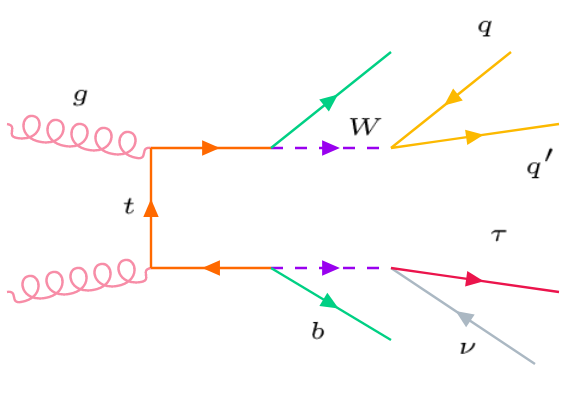
\includegraphics[width=.33\textwidth]{DiHiggs/plots/feynman_ttbarfakes.png} \hspace{2cm}
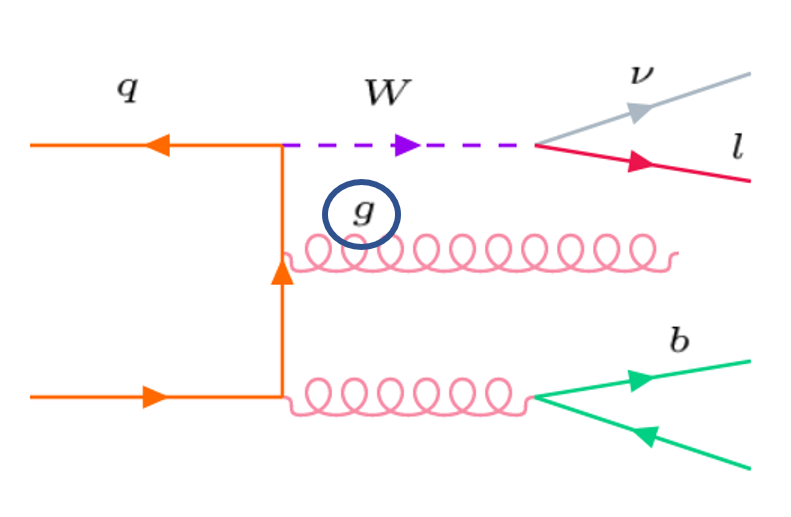
\includegraphics[width=.33\textwidth]{DiHiggs/plots/feynman_QCDfakes.png}
\caption{
Feynman diagrams on the left (right) for the \ttbar\ (multi-jet) with quark (gluon) circled in
red (blue) misidentified as a \tauhad. 
}
\label{fig:fakes:feynman}
\end{figure} 

\subsubsection{Fake factor method}
The fake-\tauhad\ background events
are estimated using a data-driven method due to imperfect MC modelling of these processes:
the `fake factor' (FF) method.
In short, the FF is the ratio of 
the number of events with fake-\tauhad\ in one region to another region.
In this analysis, 
the numerator of the FF is the number of fake-\tauhad\ events 
passing the nominal Tau-ID selection (referred to as ID selection), 
and the denominator is the number of fake-\tauhad\ events passing the
anti-\tauhad\ selection (referred to as anti-ID selection, 
as defined in detail in Section~\ref{sec:antitau-selection}). 
The fake factors are calculated in different control regions, and
then used to normalise the fake-\tauhad\ events from the 
anti-\tauhad\ selection to the signal region selection. 

In formula form, the FF is given as:
\begin{equation}
\mathrm{FF} =  \frac{N(ID selection)}{N(anti-ID selection),} 
\end{equation} 
and to obtain the estimation of the $N(ID selection)$ ($N(anti-ID selection)$),
events with a true \tauhad\ are subtracted from the data events
passing the ID (anti-ID) selection.

Due to the different origins of the fake-\tauhad, the FFs are
calculated separately for the \ttbar\ and multi-jet, 
and for 1 and 3-prong \tauhad\ candidates.
The FF is parameterised in bins of \pt\ of the \tauhad, while the 
dependence on $\eta$ is also checked but no obvious trend is observed.
For each process the $FF$ are calculated in 
a dedicated background enriched region (FF-CR,
not to be confused with the CR used for statistical analysis). 
The FF-CRs for each process are defined as follows:
\begin{itemize}
\item \ttbar\ FF-CR: same selection as the signal region selection 
but with \mbb\ cut reversed: \mbb\ > 150 GeV.
\item Multi-jet (QCD) FF-CR: same selection as the signal region selection lepton isolation requirements
 reversed: `tight' electrons and `medium' muons are required to fail 
 their respective `loose' isolation working points.
\end{itemize}

Individual fake factors for each process
are then used to provide a combined fake factor. 
The combined $FF$ is finally applied to the events passing the 
anti-ID selection
to estimate the fake-\tauhad\ events in the SR.
The FFs are derived separately for the SLT and LTT channels and
so is the fake background estimation in the SR.
The combined fake factor is defined as:
\begin{equation}
FF(\mathrm{comb}) = FF(\mathrm{QCD}) \times \mathrm{r}_{\mathrm{QCD}} + FF(\ttbar) \times (1 - \mathrm{r}_{\mathrm{QCD}}),
\end{equation} 
where the $FF(\mathrm{QCD})$ ($FF(\ttbar)$) is the FF calculated in the QCD (\ttbar) FF-CR.
The $\mathrm{r}_{\mathrm{QCD}}$ is
defined as the fraction of QCD fakes
in the total number of fake-\tauhad\ background, 
where it is measured as a function of the \tauhad\ \pT, splitted 
into 1-prong and 3-prong, and into the type of light lepton ($e$ or $mu$)
since the QCD contents are different for them. 
The $\mathrm{r}_{\mathrm{QCD}}$ is measured for events passing the 
anti-ID selection, and the formula form is:
\begin{equation}
\mathrm{r}_{\mathrm{QCD}} = \frac{N(\mathrm{multi\mhyphen jet, data})} {N(\mathrm{data}) - N(\mathrm{true}~\tauhad, \mathrm{MC})}
\end{equation} 
and the $N(\mathrm{multi\mhyphen jet, data})$ is calculated by 
subtracting all background contributions apart from multi-jet, 
regardless of whether they contain fake or true-\tauhad\ candidates, 
from the data in the anti-\tauhad\ selection:
\begin{equation}
	N(\mathrm{multi\mhyphen jet, data}) = N(\mathrm{data}) - N(\mathrm{true}~\tauhad, \mathrm{MC}) - N(\mathrm{fake}~\tauhad, \mathrm{MC})
\end{equation}  
The subtracted backgrounds are taken from the MC predictions,
and the MC simulated fake background has solely the contribution from the
\ttbar\ fakes. 


In graphical form, the various FF-CRs 
where the fake factors are measured and applied can be seen in Figure~\ref{fig:CombFFMethod}.
\begin{figure}[htbp]
\centering
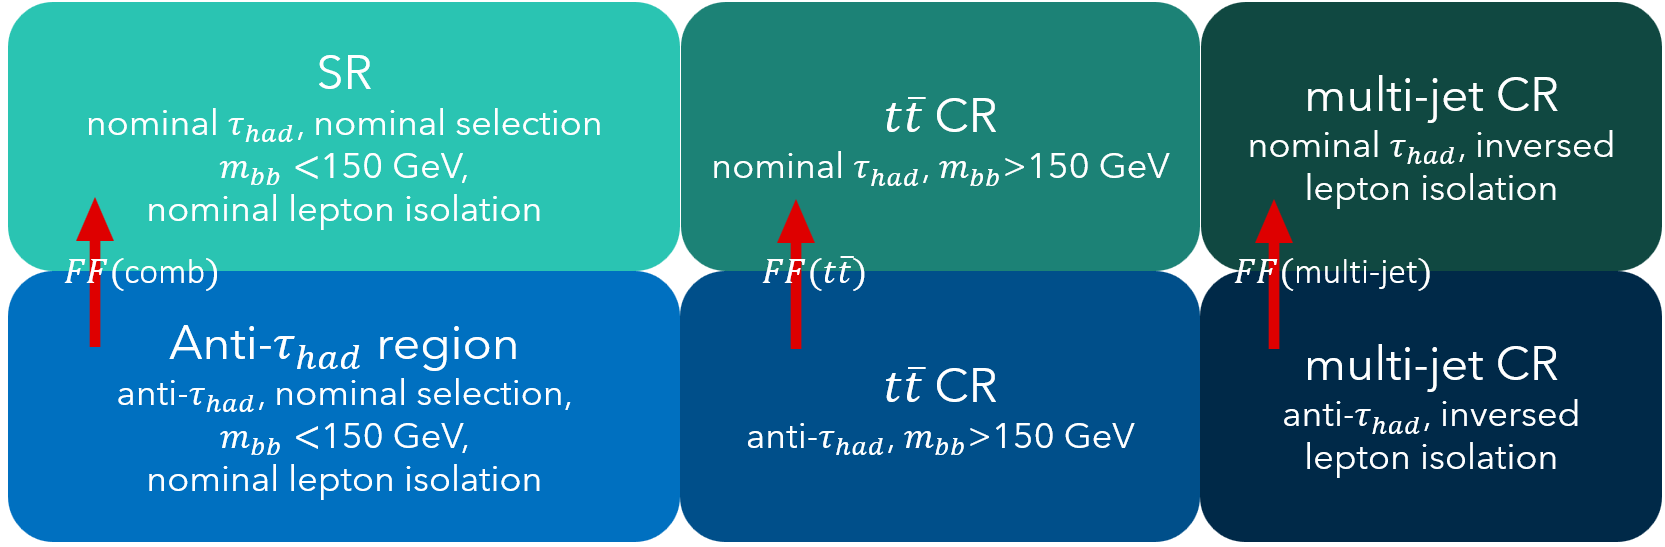
\includegraphics[width=.9\textwidth]{DiHiggs/plots/FF regions.png}
\caption{Graphical representation of the Combined Fake Factor Method. 
The fake factors are calculated independently for the \ttbar\ FF-CR and the multi-jet FF-CR, and 
combined to the combined fake factor. 
The direction of the arrow indicates the direction 
of extrapolation, 
that the FF is applied on the bottom regions to extrapolate to the top regions.}
\label{fig:CombFFMethod}
\end{figure}



\subsubsection{\ttbar\ background reweighting}
\label{sec:ttbar-reweighting}
The determination of the combined fake factor 
is sensitive to the modelling of simulated $t\bar{t}$ events with true-\tauhad\
given that this is the dominant background that is subtracted from data in the derivation of
the FFs and $\mathrm{r}_\text{QCD}$, and when obtaining the events passing the ID. 
Additionally, the derivation of $\mathrm{r}_\text{QCD}$ is sensitive to the 
modelling of simulated $t\bar{t}$ events with fake-\tauhad.
It was observed that mismodeling in the true \ttbar\ background 
especially in the high jet multiplicity and high top-quark \pt\ 
can cause issues in the calculation of the fake factors, 
giving non-physical negative values at high \tauhad\ \pt\ region. 
To mitigate this issue,
simulated events from $t\bar{t}$ production are differentially reweighted
depending on the jet multiplicity and the scalar sum of the transverse momentum of all visible
final state objects ($H_T$) in the event.

These reweighting factors are determined bin-by-bin 
in distribution of jet multiplicity and $H_T$,
from another $t\bar{t}$ FF-CR ($t\bar{t}$ FF-CR2),
% which is about 93\% pure in the events from $t\bar{t}$ production,
which is defined using a selection identical to the SR selection,
but with the \ttbar\ FF-CR $m_{bb}$ requirements ($m_{bb}>150$~GeV)
and an additional $m^{W}_\text{T}>40$~GeV requirement. 
Furthermore, events in this region are required
to have a reconstructed \tauhad\ candidate, but this candidate is not required
to pass any RNN \tauhad\ requirement.
The $m^{W}_\text{T}$ requirement is introduced to remove any potential contamination from multi-jet events.
The reweighting factors are shown in Appendix~\ref{sec:appendix:fakes}, 
Figure~\ref{fig:ttbarReweighting_parametrisations}

The reweighting method is validated in two additional validation regions.
The reweighting only applies to the fake-background estimation process
%  FF-CRs,  and the anti-\tauhad\ regions, 
while it's not applyied to the true \ttbar\ background in the SR, 
as there is no significant mismodeling seen there, and
the uncertainties due to the \ttbar\ modelling has been taken care differently 
(more details in section~TODO: ref back to systematics section\ref{fig:}).   
% it would complicate the \ttbar\ systematics uncertainties and statistical analysis.


\subsubsection{Fake factor calculation}
The data and MC events in \ttbar\ FF-CR passing the anti-ID selection 
before and after the \ttbar\ reweighting 
are shown in Figure~\ref{fig:ttbarCR_1} and \ref{fig:ttbarCR_3}, respectively.
The fake background is simulated by MC, and only includes 
the contributions from the \ttbar\ fakes. 
A clear mismodeling can be seen in the plots before 
the reweighting, and it is much mitigated after the 
reweighting process. At this stage, data and MC are 
not expected to agree well due to the \ttbar\ fake is known to
be poorly modelled by the MC. 
Nevertheless, a large number of \ttbar\ fakes is observed, suggesting
the high purity of \ttbar\ fakes in this region. 
With true \tauhad\ contributions subtracted from the data 
(and with true \tauhad\ \ttbar\ reweighted),  
this region is used as the denominator of the \ttbar\ FF-CR fake factor calculation. 




\begin{figure}[htbp]
\centering
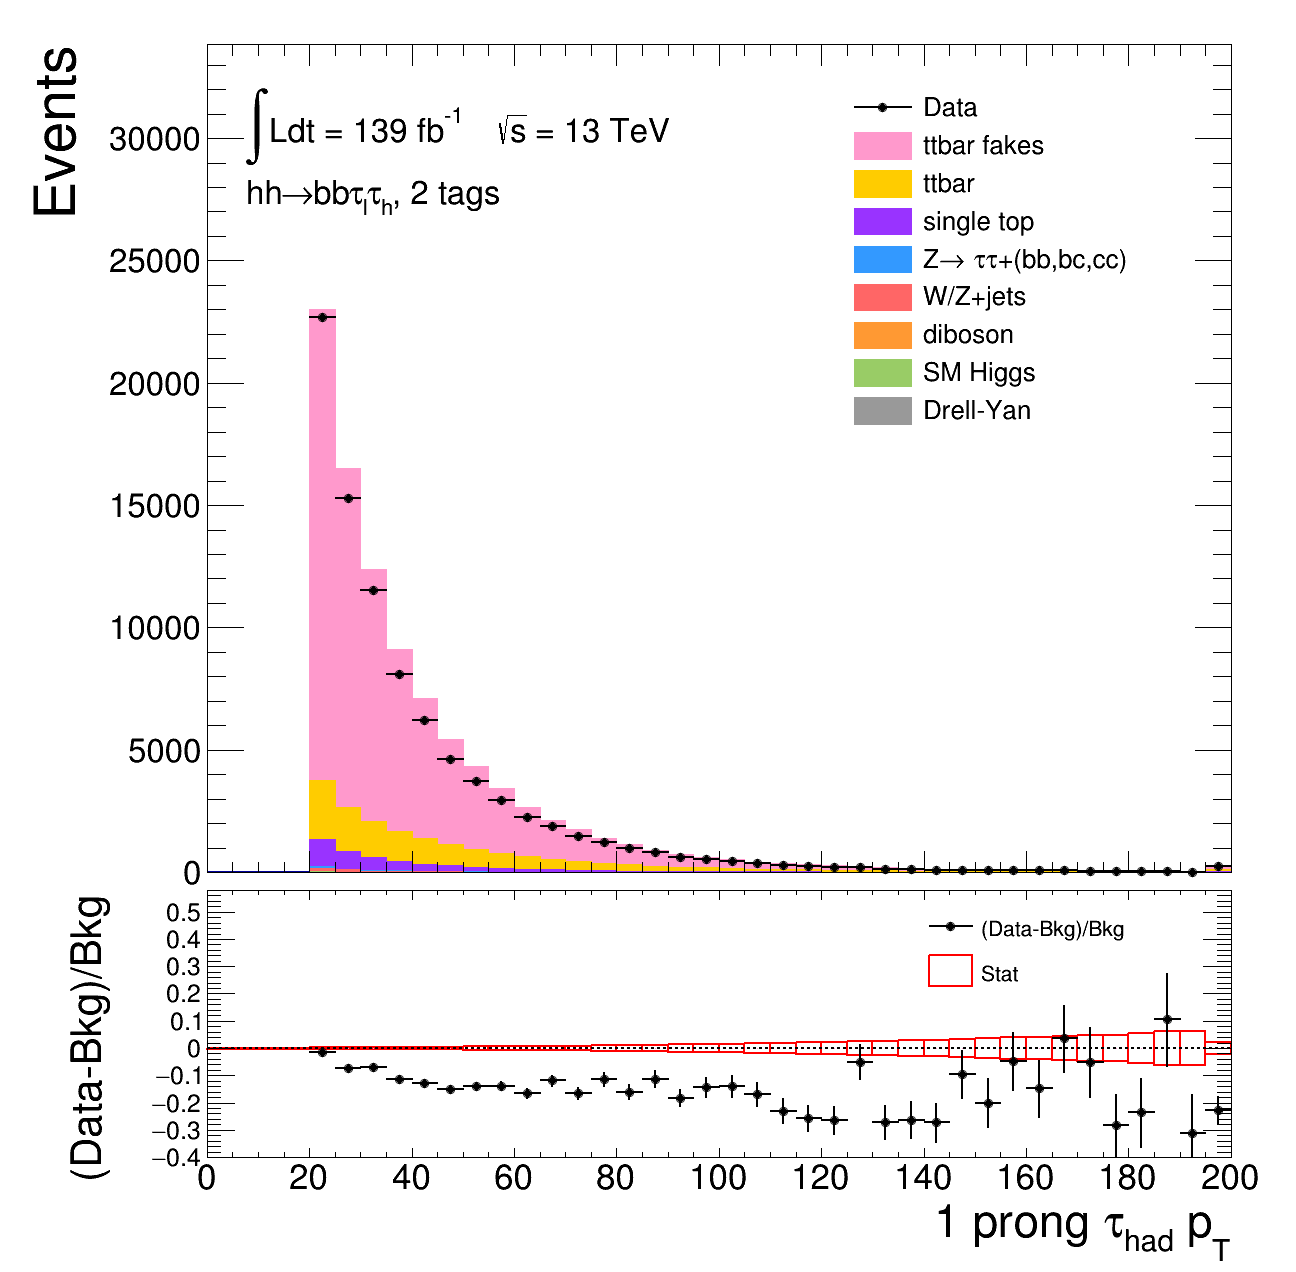
\includegraphics[width=.45\textwidth]{DiHiggs/plots/FF_CRs/ttbarCR_SLT/HNone/BDTVarsHighMbb/2/C_2tag2pjet_0ptv_TauPt1P.png}
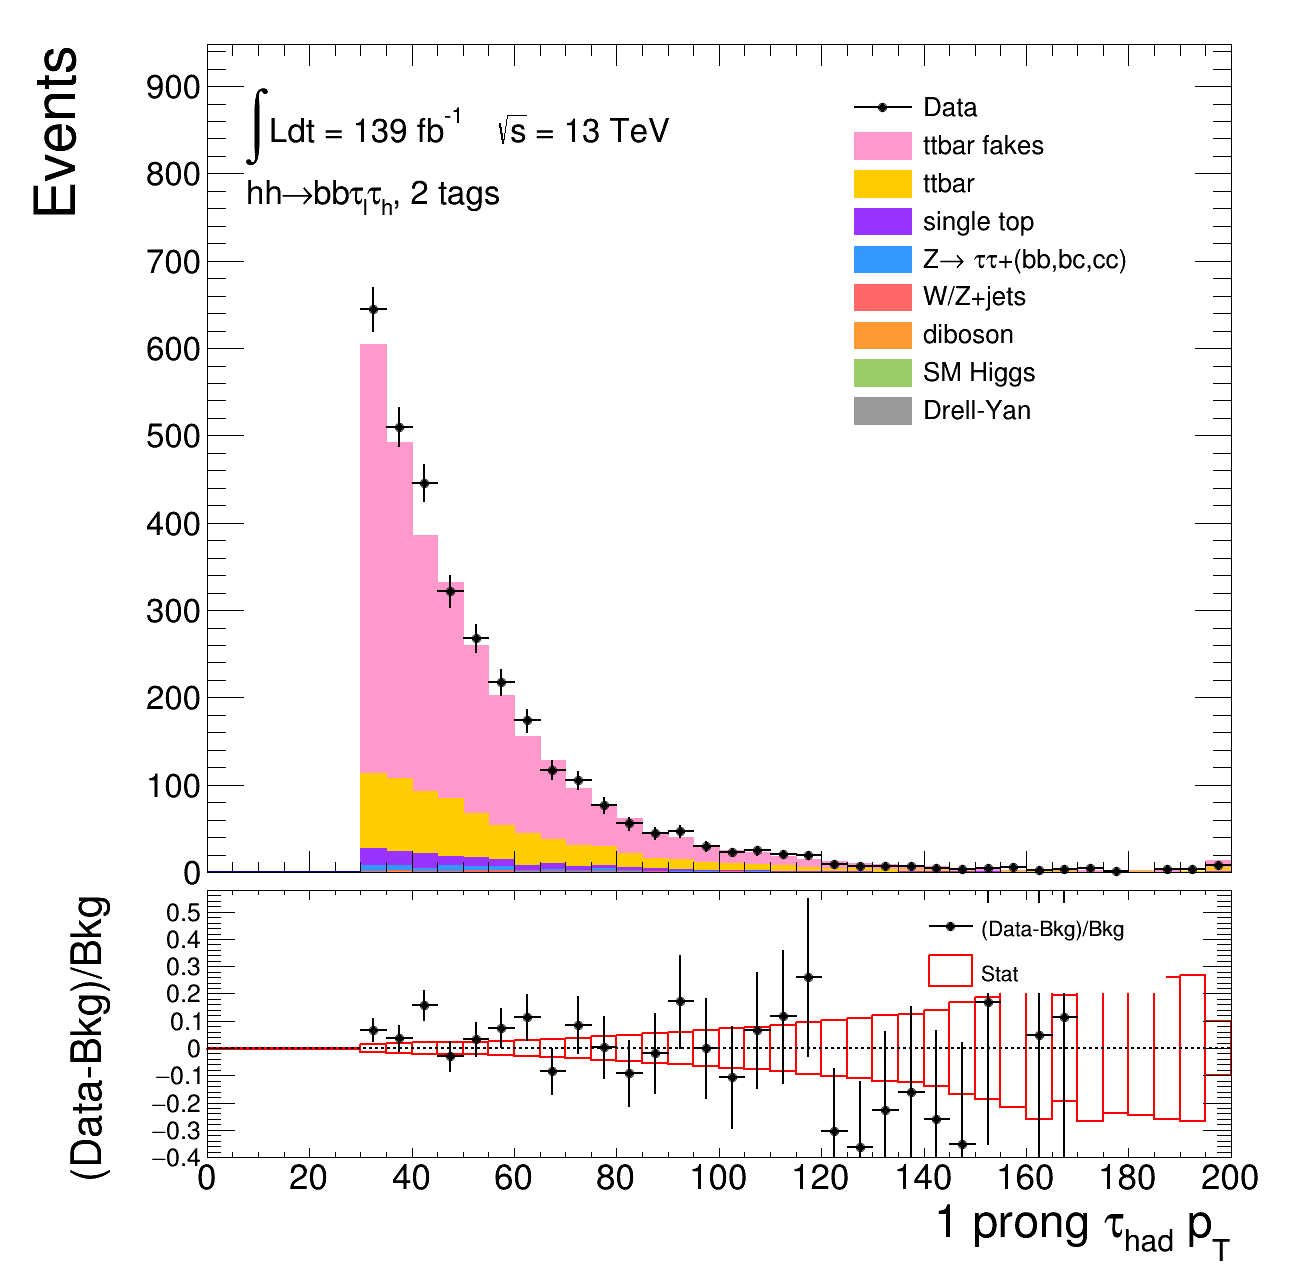
\includegraphics[width=.45\textwidth]{DiHiggs/plots/FF_CRs/ttbarCR_LTT/HNone/BDTVarsHighMbb/2/C_2tag2pjet_0ptv_TauPt1P.png}\\
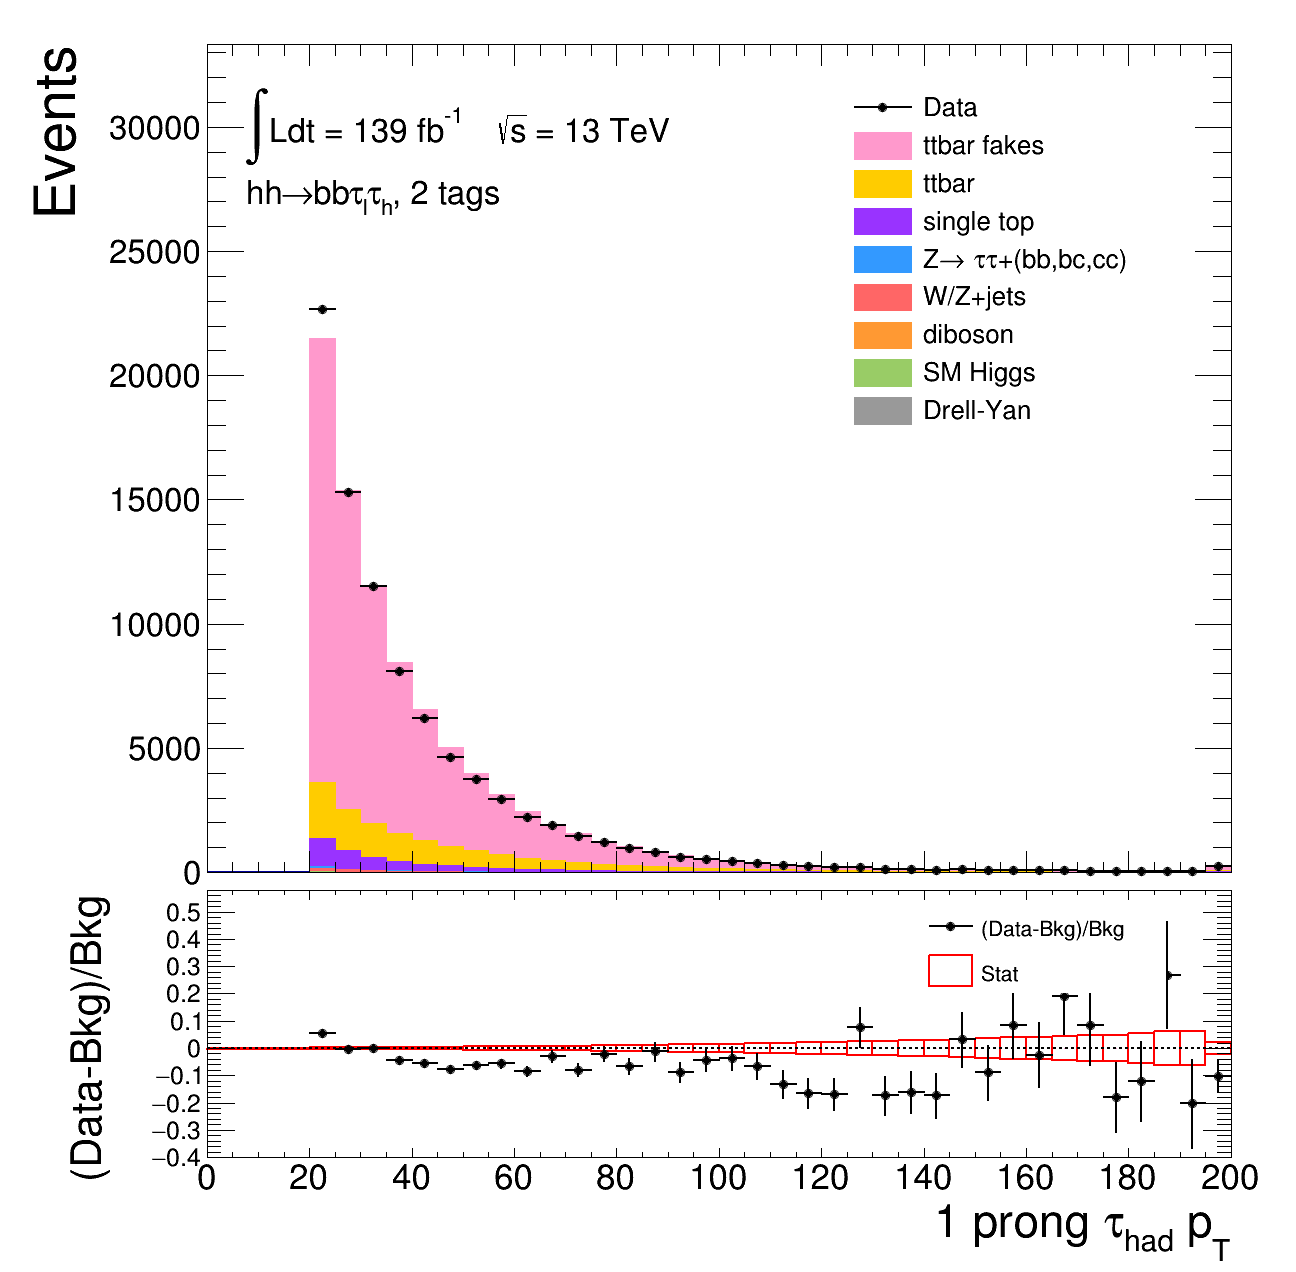
\includegraphics[width=.45\textwidth]{DiHiggs/plots/FF_CRs/ttbarCR_SLT_weighted/HNone/BDTVarsHighMbb/2/C_2tag2pjet_0ptv_TauPt1P.png}
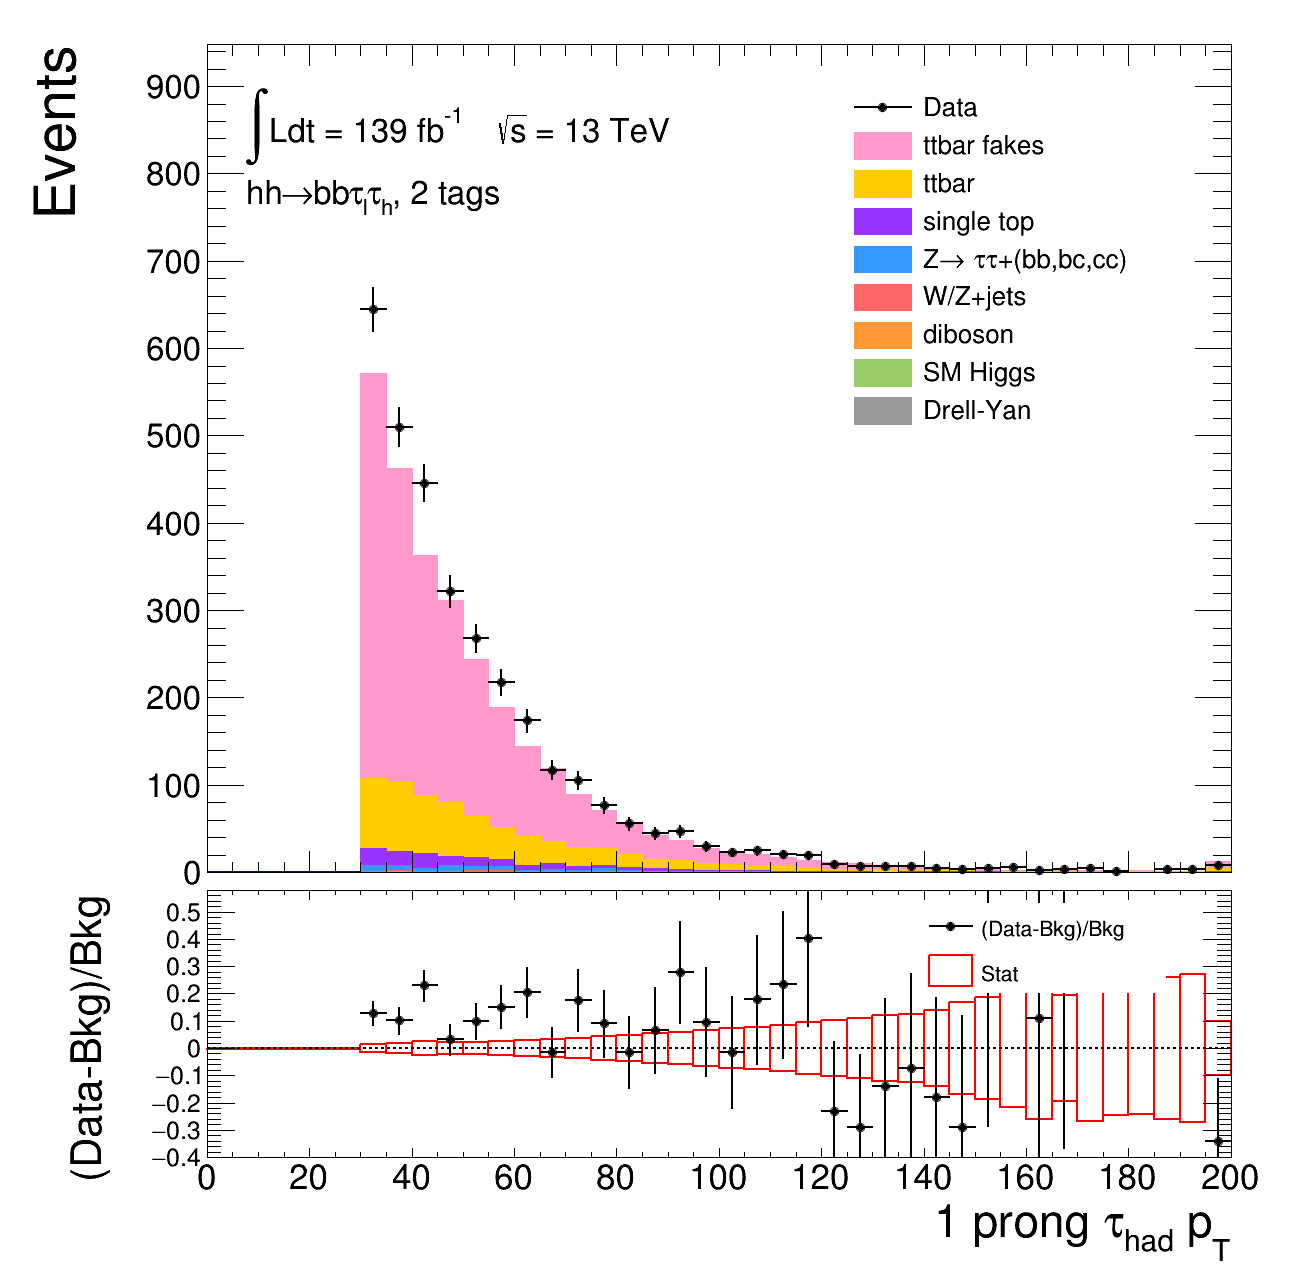
\includegraphics[width=.45\textwidth]{DiHiggs/plots/FF_CRs/ttbarCR_LTT_weighted/HNone/BDTVarsHighMbb/2/C_2tag2pjet_0ptv_TauPt1P.png}\\
\caption{In the \ttbar\ FF-CR, the $\tauhad$ $p_T$ distributions are plotted 
for the SLT (left) and LTT channel (right) 
with \ttbar\ un-weighted (top) 
and with \ttbar\ re-weighted (bottom).
The \tauhad\ in these events have 1 prong. 
The \ttbar\ fakes is labelled as `ttbar fakes' in pink.
Only statistical uncertainty is considered.}
\label{fig:ttbarCR_1}
\end{figure} 
\begin{figure}[htbp]
\centering
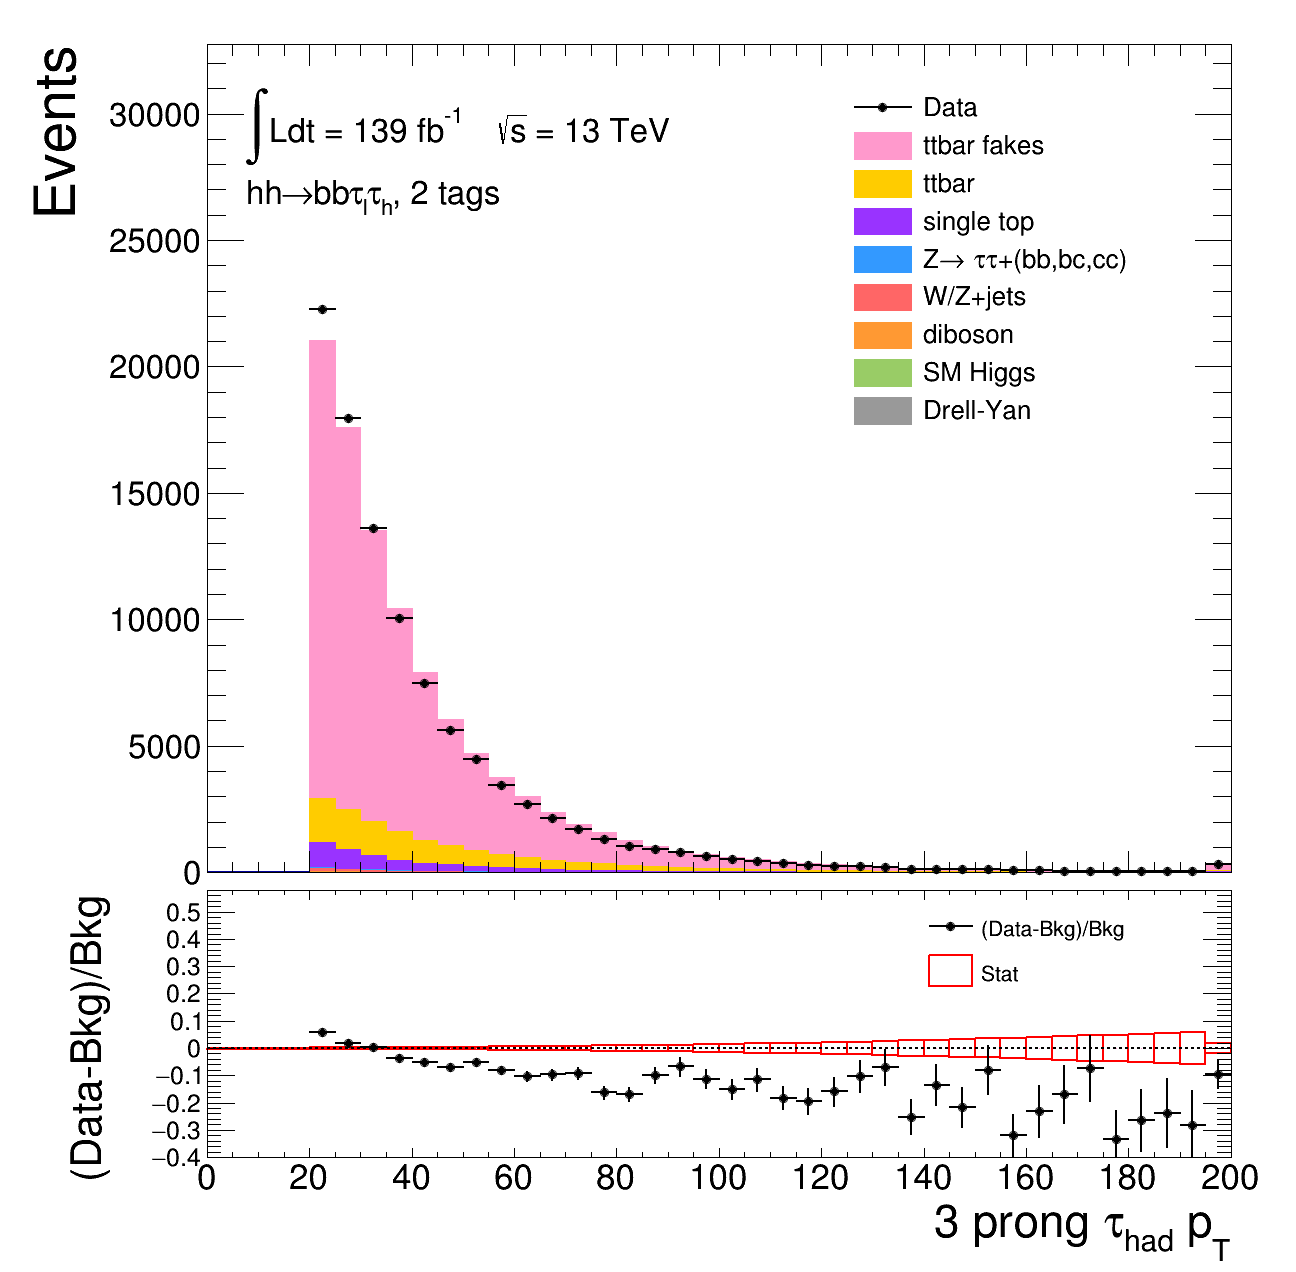
\includegraphics[width=.45\textwidth]{DiHiggs/plots/FF_CRs/ttbarCR_SLT/HNone/BDTVarsHighMbb/2/C_2tag2pjet_0ptv_TauPt3P.png}
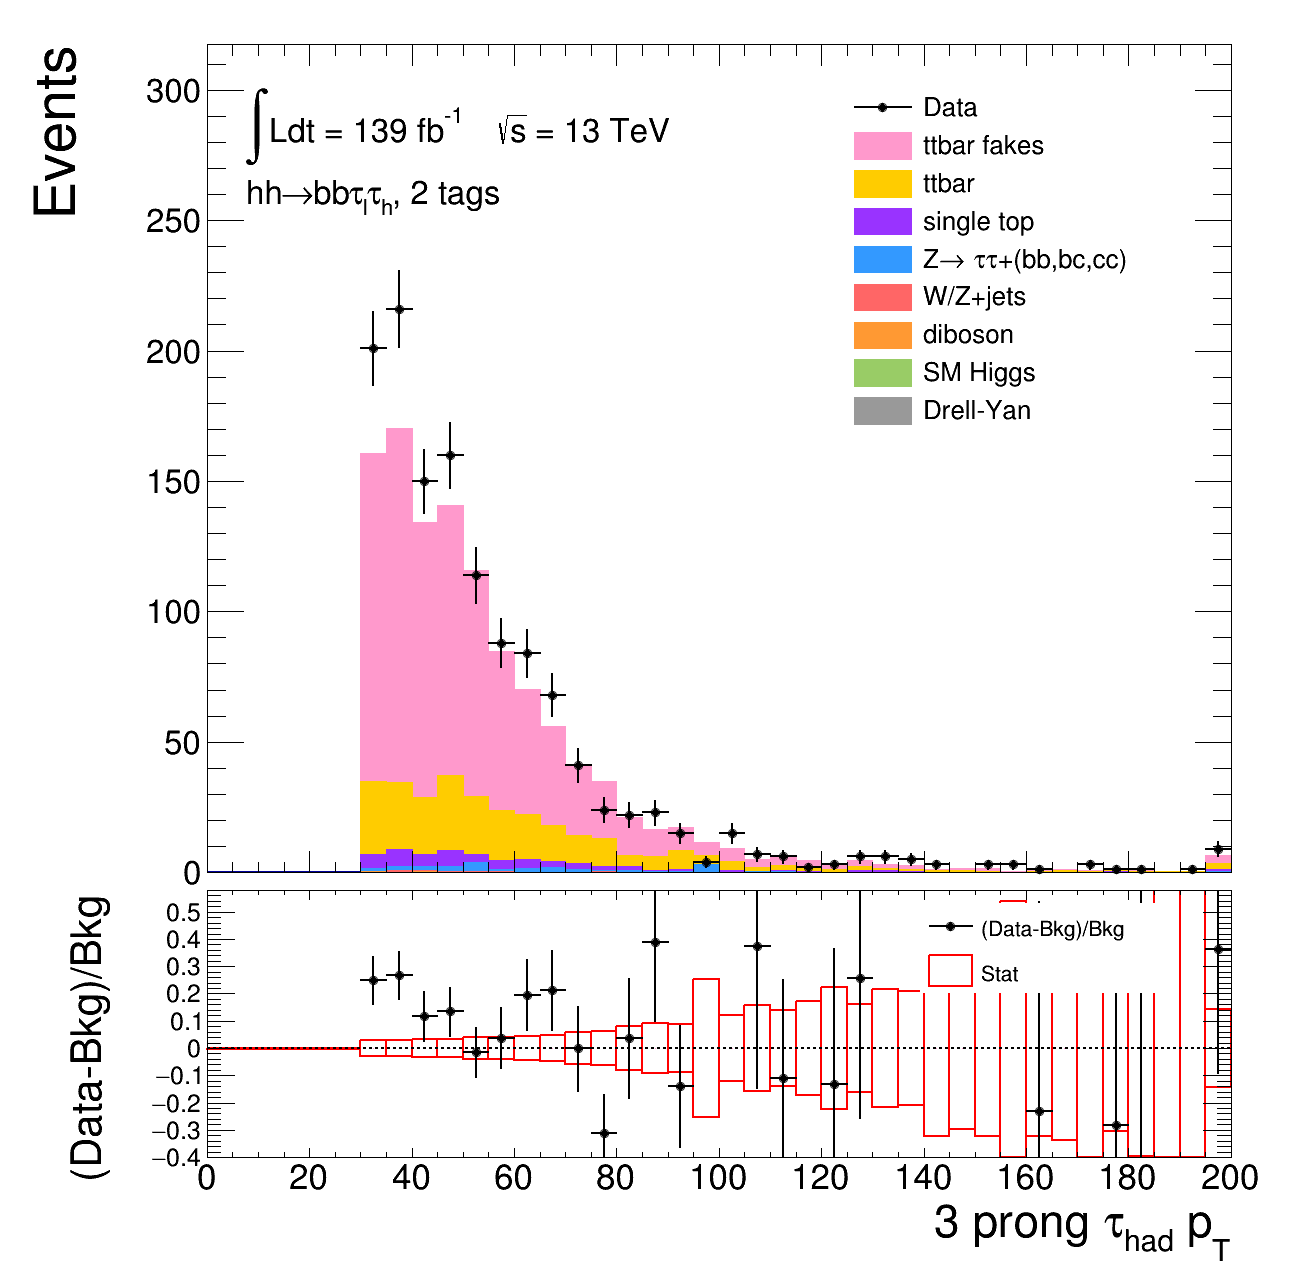
\includegraphics[width=.45\textwidth]{DiHiggs/plots/FF_CRs/ttbarCR_LTT/HNone/BDTVarsHighMbb/2/C_2tag2pjet_0ptv_TauPt3P.png}\\
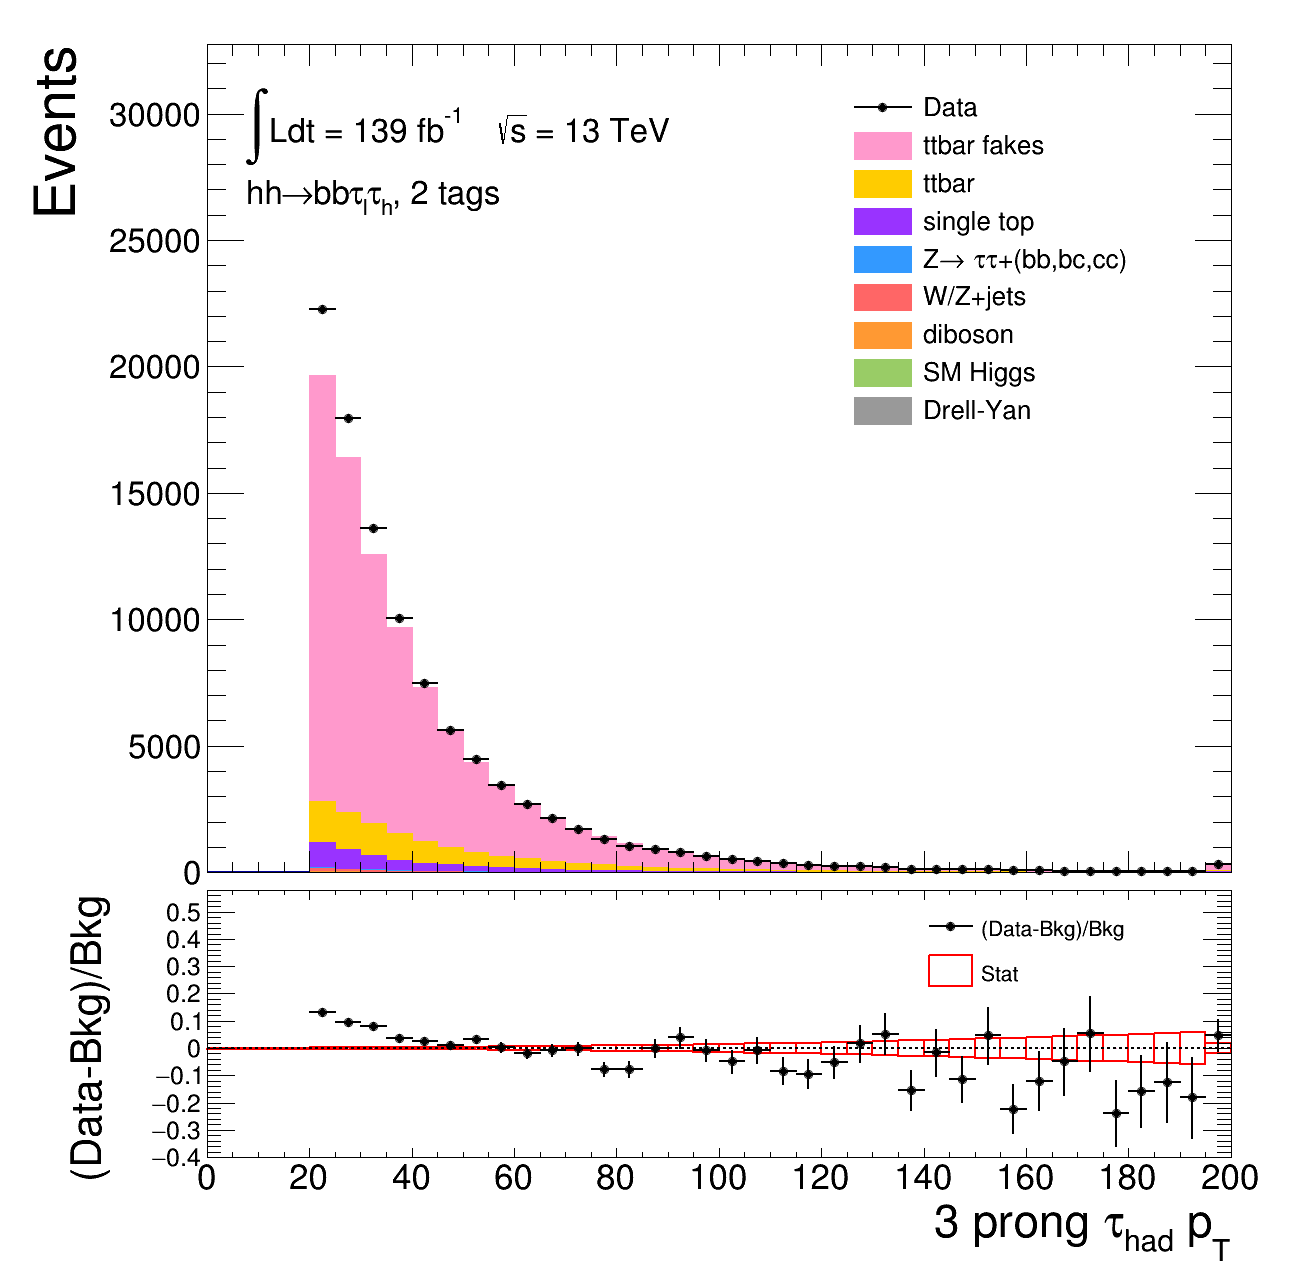
\includegraphics[width=.45\textwidth]{DiHiggs/plots/FF_CRs/ttbarCR_SLT_weighted/HNone/BDTVarsHighMbb/2/C_2tag2pjet_0ptv_TauPt3P.png}
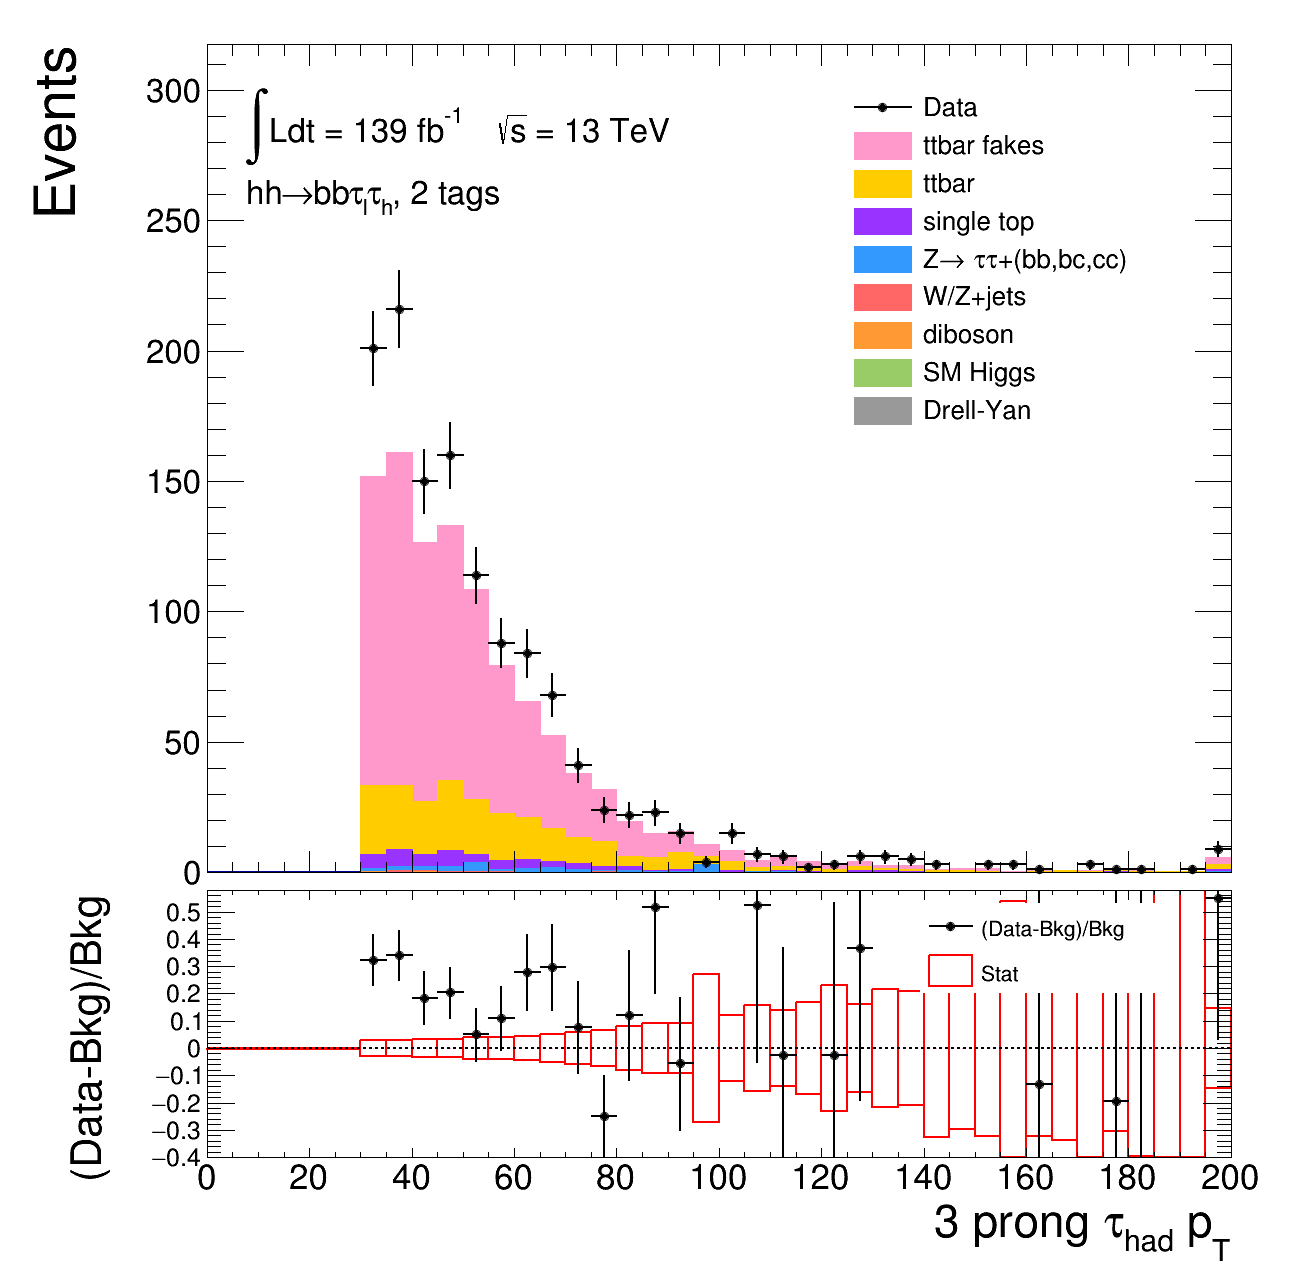
\includegraphics[width=.45\textwidth]{DiHiggs/plots/FF_CRs/ttbarCR_LTT_weighted/HNone/BDTVarsHighMbb/2/C_2tag2pjet_0ptv_TauPt3P.png}\\
\caption{In the \ttbar\ FF-CR, the $\tauhad$ $p_T$ distributions are plotted 
for the SLT (left) and LTT channel (right) 
with \ttbar\ un-weighted (top) 
and with \ttbar\ re-weighted (bottom).
The \tauhad\ in these events have 3 prongs. 
The \ttbar\ fakes is labelled as `ttbar fakes' in pink.
Only statistical uncertainty is considered.
}
\label{fig:ttbarCR_3}
\end{figure} 



Similarly, the data and MC events in QCD FF-CR passing the anti-ID selection 
before and after the \ttbar\ reweighting 
\ref{fig:InvCR_1} and \ref{fig:InvCR_3}, respectively.
Since the QCD fakes is not modelled by the MC, a large discrepancy
is shown between data and the MC distributions, which is comprised
of the QCD fakes. 
For consistency, the \ttbar\ reweighting is applied, 
however, this region is dominated 
by the QCD fakes and the \ttbar\ contributions is negligible. 
The contribution from \ttbar\ fakes is also very small, suggesting 
the purity of QCD fakes is high in this region. 
With true \tauhad\ contributions subtracted from data, 
this region is used as the denominator of the QCD FF-CR fake factor calculation. 

\begin{figure}[htbp]
\centering
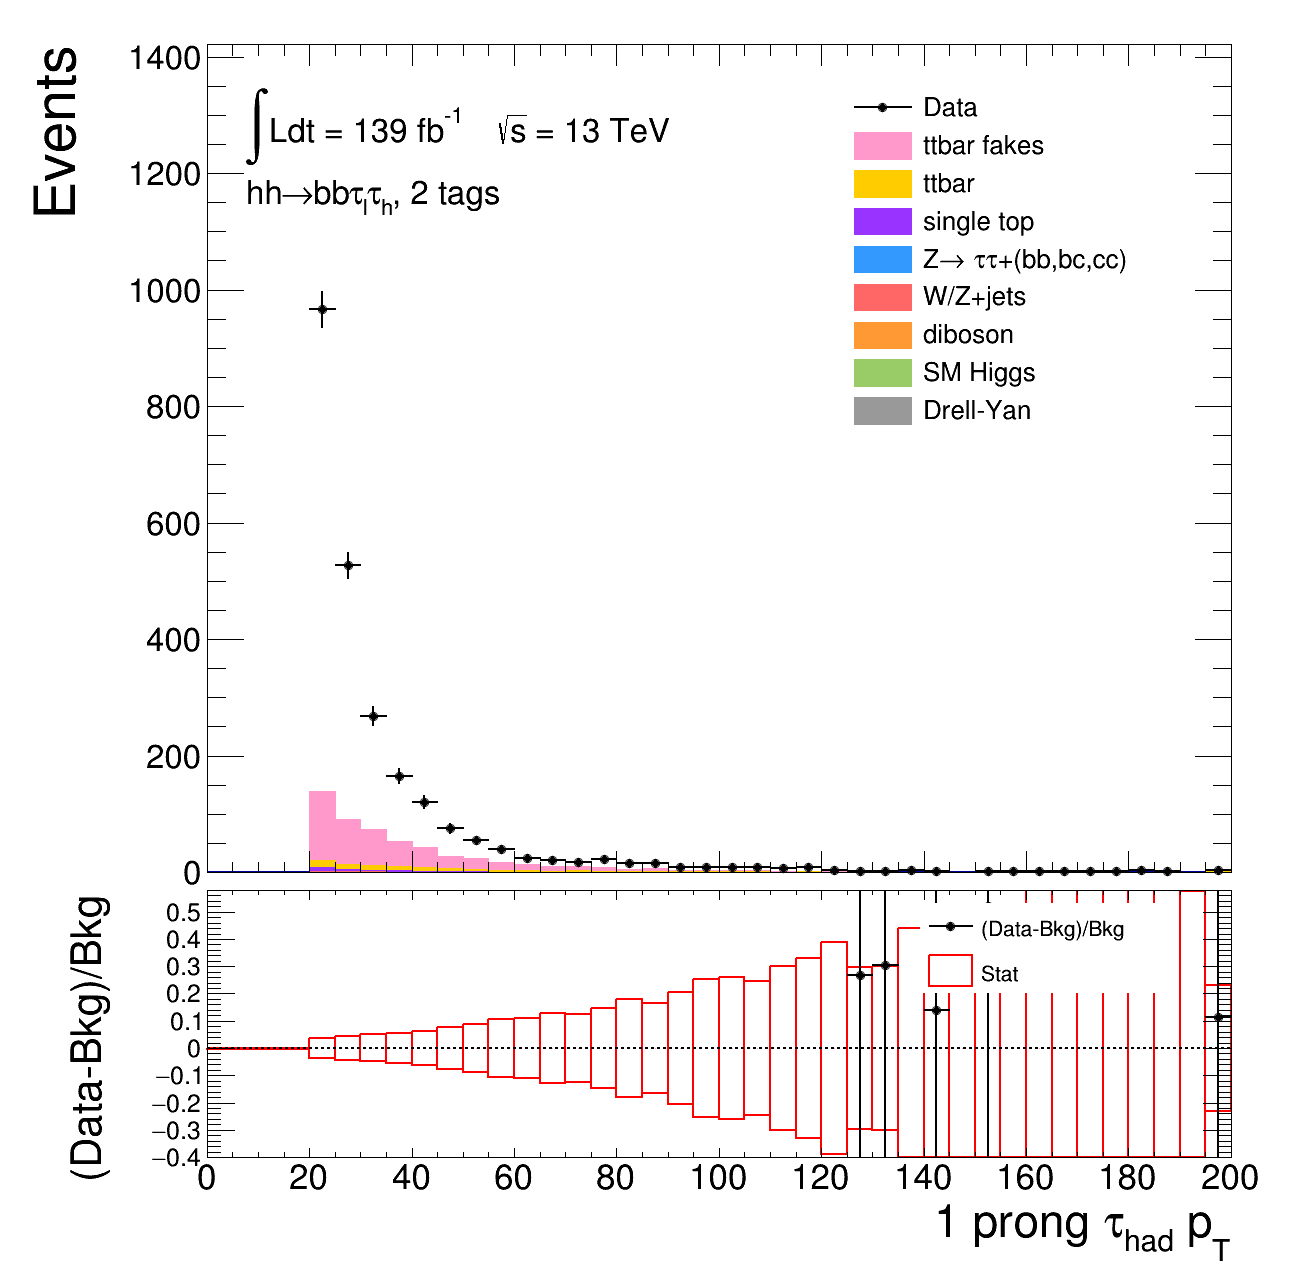
\includegraphics[width=.45\textwidth]{DiHiggs/plots/FF_CRs/InvCR_SLT/HNone/BDTVarsHighMbb/2/C_2tag2pjet_0ptv_TauPt1P.png}
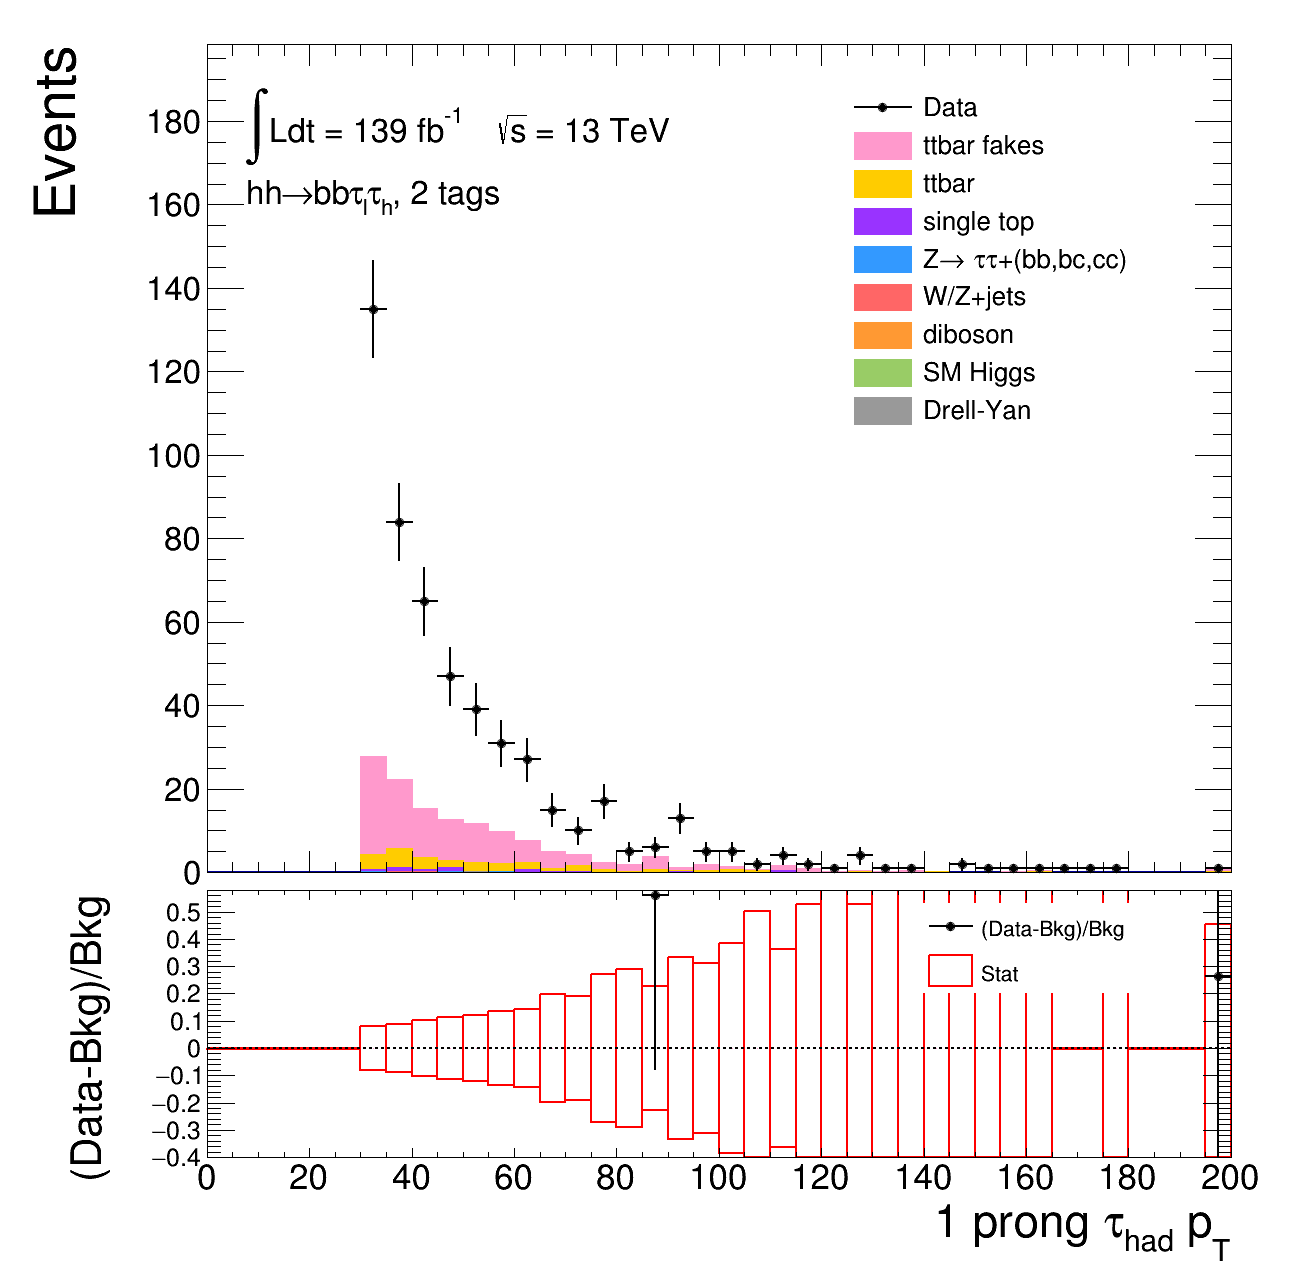
\includegraphics[width=.45\textwidth]{DiHiggs/plots/FF_CRs/InvCR_LTT/HNone/BDTVarsHighMbb/2/C_2tag2pjet_0ptv_TauPt1P.png}\\
\caption{In the QCD FF-CR, the $\tauhad$ $p_T$ distributions are plotted 
for the SLT (left) and LTT channel (right) 
with \ttbar\ re-weighted.
The \tauhad\ in these events have 1 prong. 
The \ttbar\ fakes is labelled as `ttbar fakes' in pink.
Only statistical uncertainty is considered.}
\label{fig:InvCR_1}
\end{figure} 

\begin{figure}[htbp]
\centering
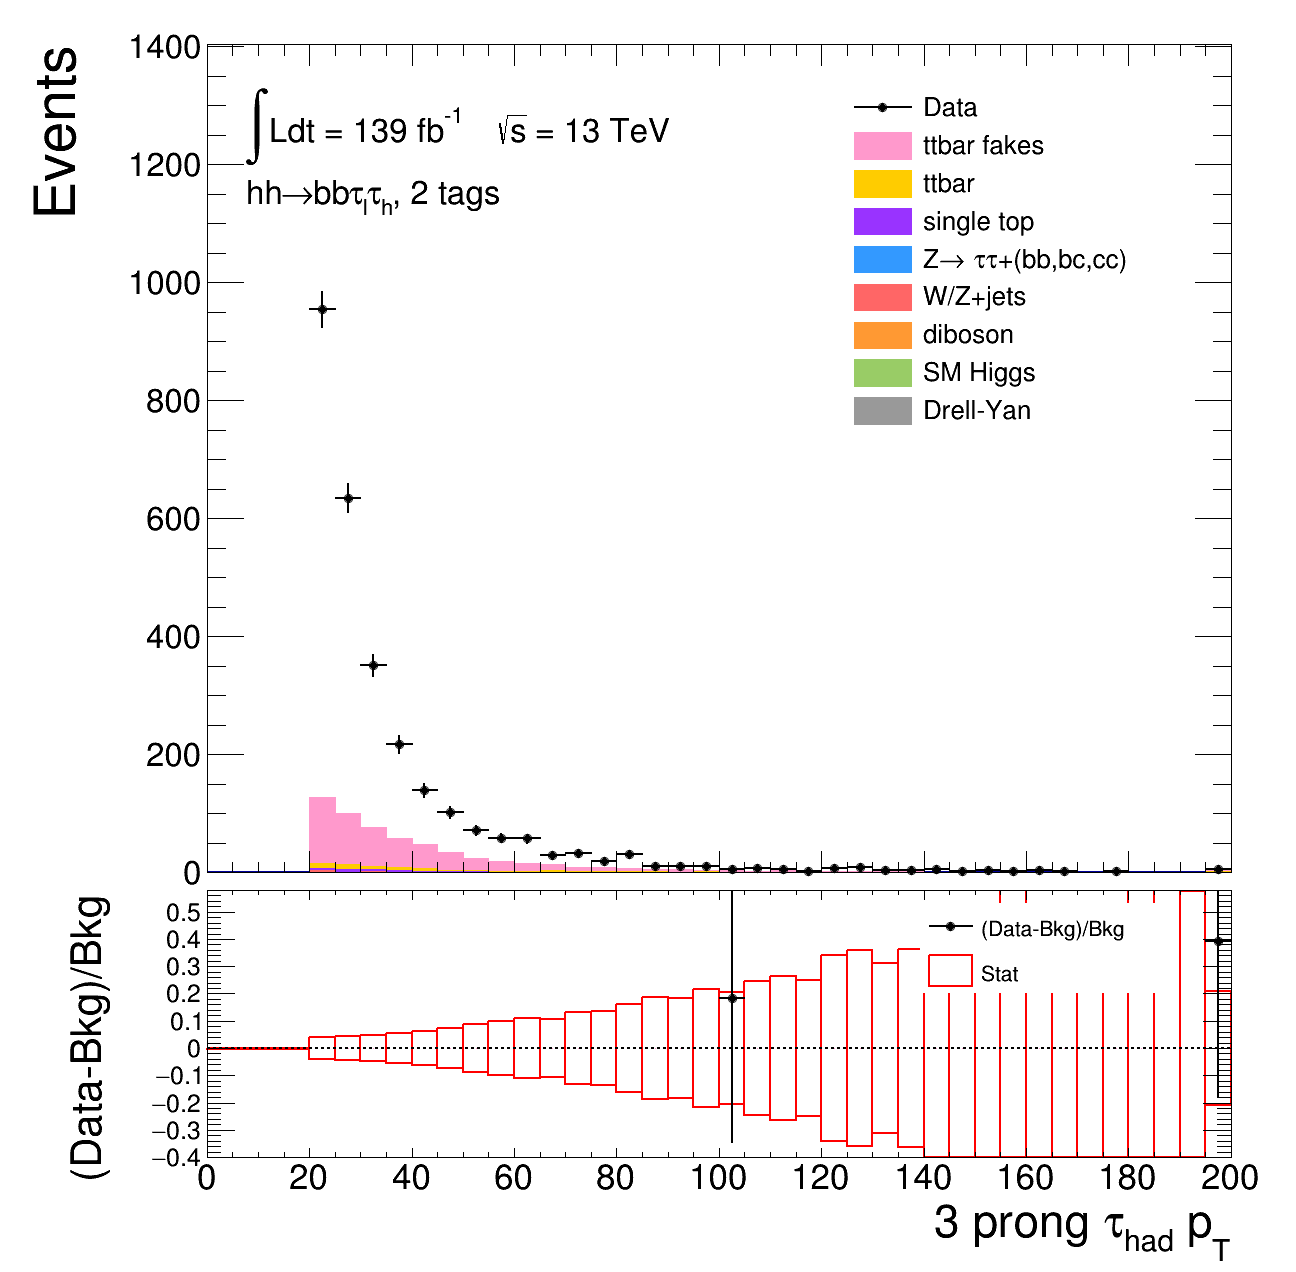
\includegraphics[width=.45\textwidth]{DiHiggs/plots/FF_CRs/InvCR_SLT/HNone/BDTVarsHighMbb/2/C_2tag2pjet_0ptv_TauPt3P.png}
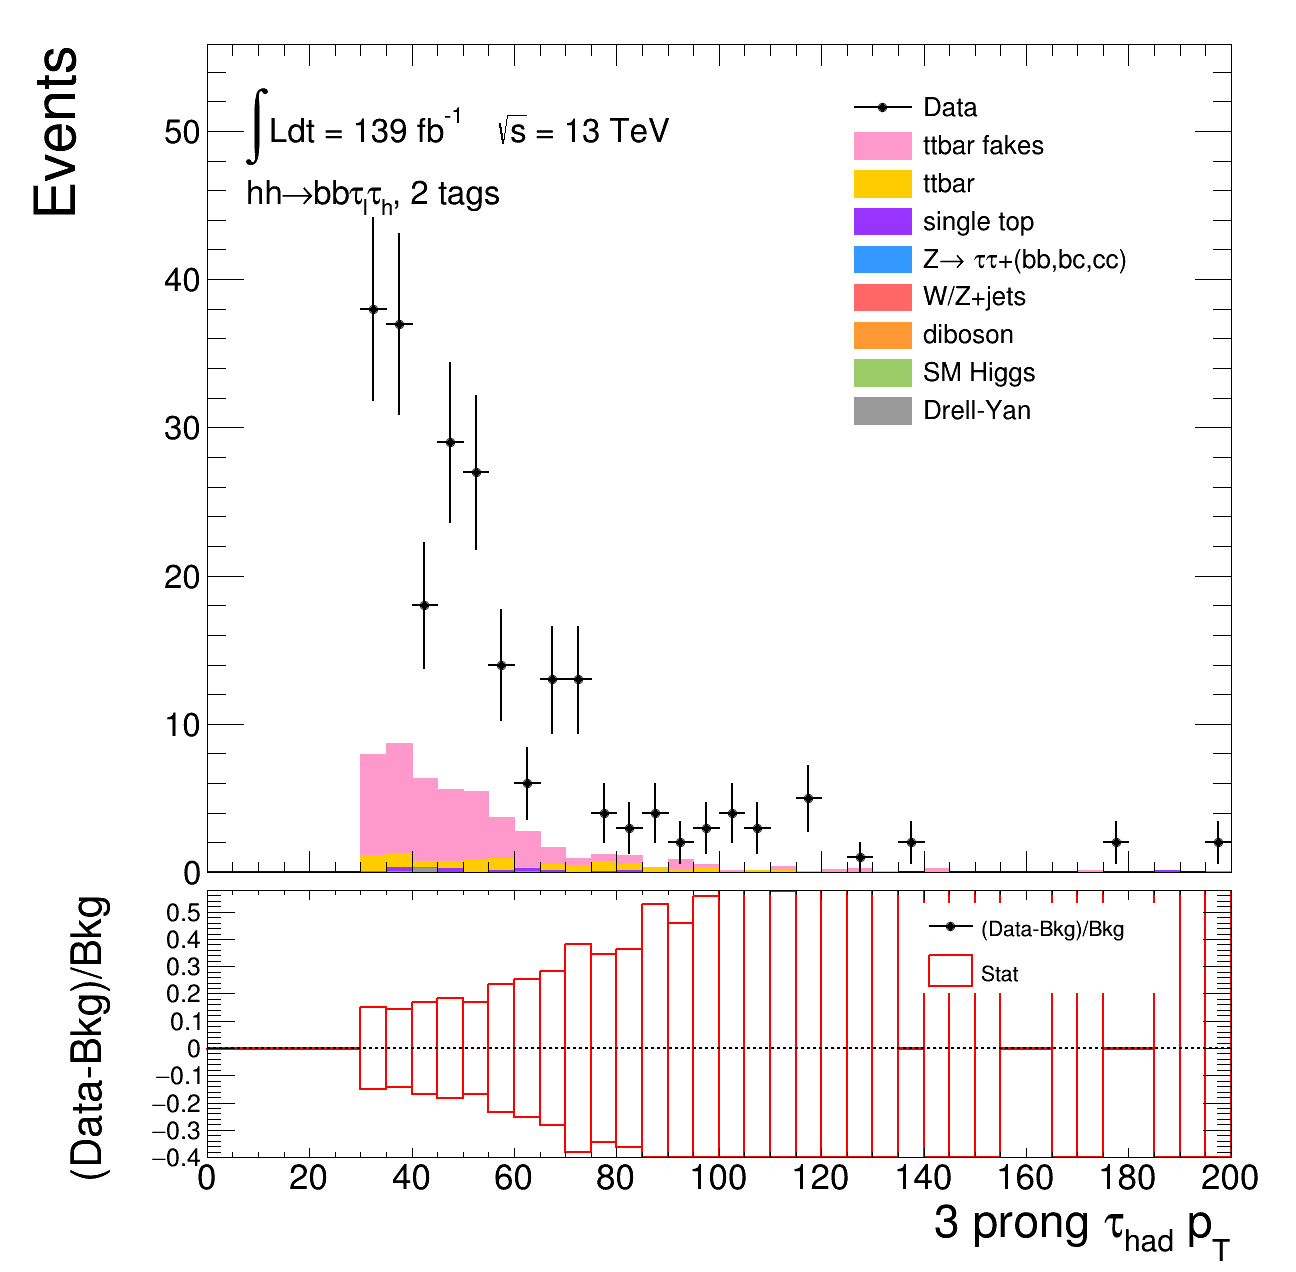
\includegraphics[width=.45\textwidth]{DiHiggs/plots/FF_CRs/InvCR_LTT/HNone/BDTVarsHighMbb/2/C_2tag2pjet_0ptv_TauPt3P.png}\\
\caption{In the QCD FF-CR, the $\tauhad$ $p_T$ distributions are plotted 
for the SLT (left) and LTT channel (right) 
with \ttbar\ re-weighted.
The \tauhad\ in these events have 3 prongs. 
Only statistical uncertainty is considered.}
\label{fig:InvCR_3}
\end{figure} 

The calculated fake factors are shown on Figure~\ref{fig:SLT_FF} and Figure~\ref{fig:LTT_FF}, 
for the SLT and LTT channels respectively. 
The Fake factors obtained with reweighted and un-weighted \ttbar\ contributions are shown on the
same graph. 
The binning is optimised for the $\text{FF}_{t\bar{t}}$ and the same binning is used for the 
$\text{FF}_\text{QCD}$. A smooth trend is observed in the $\text{FF}_{t\bar{t}}$, 
but some artifacts shapes at mid and high \pt\ range are showin in the $\text{FF}_\text{QCD}$.
This issue has no visible impact on the fakes estimation, because the 
the \ttbar\ FF dominates over the multi-jet FF in the combined FF which can be seen 
in the $\mathrm{r}_\text{QCD}$ distribution in Figure.~\ref{fig:SLT_rQCD} and Figure.~\ref{fig:LTT_rQCD}. 
The  $\mathrm{r}_{\mathrm{QCD}}$ 
for 1-prong and 3-prong \tauhad\ candidates in $e\tauhad$ and $\mu\tauhad$ channels 
are shown in Figure~\ref{fig:SLT_rQCD} for the SLT category and 
in Figure~\ref{fig:LTT_rQCD} for the LTT category.



\begin{figure}[htbp]
\centering
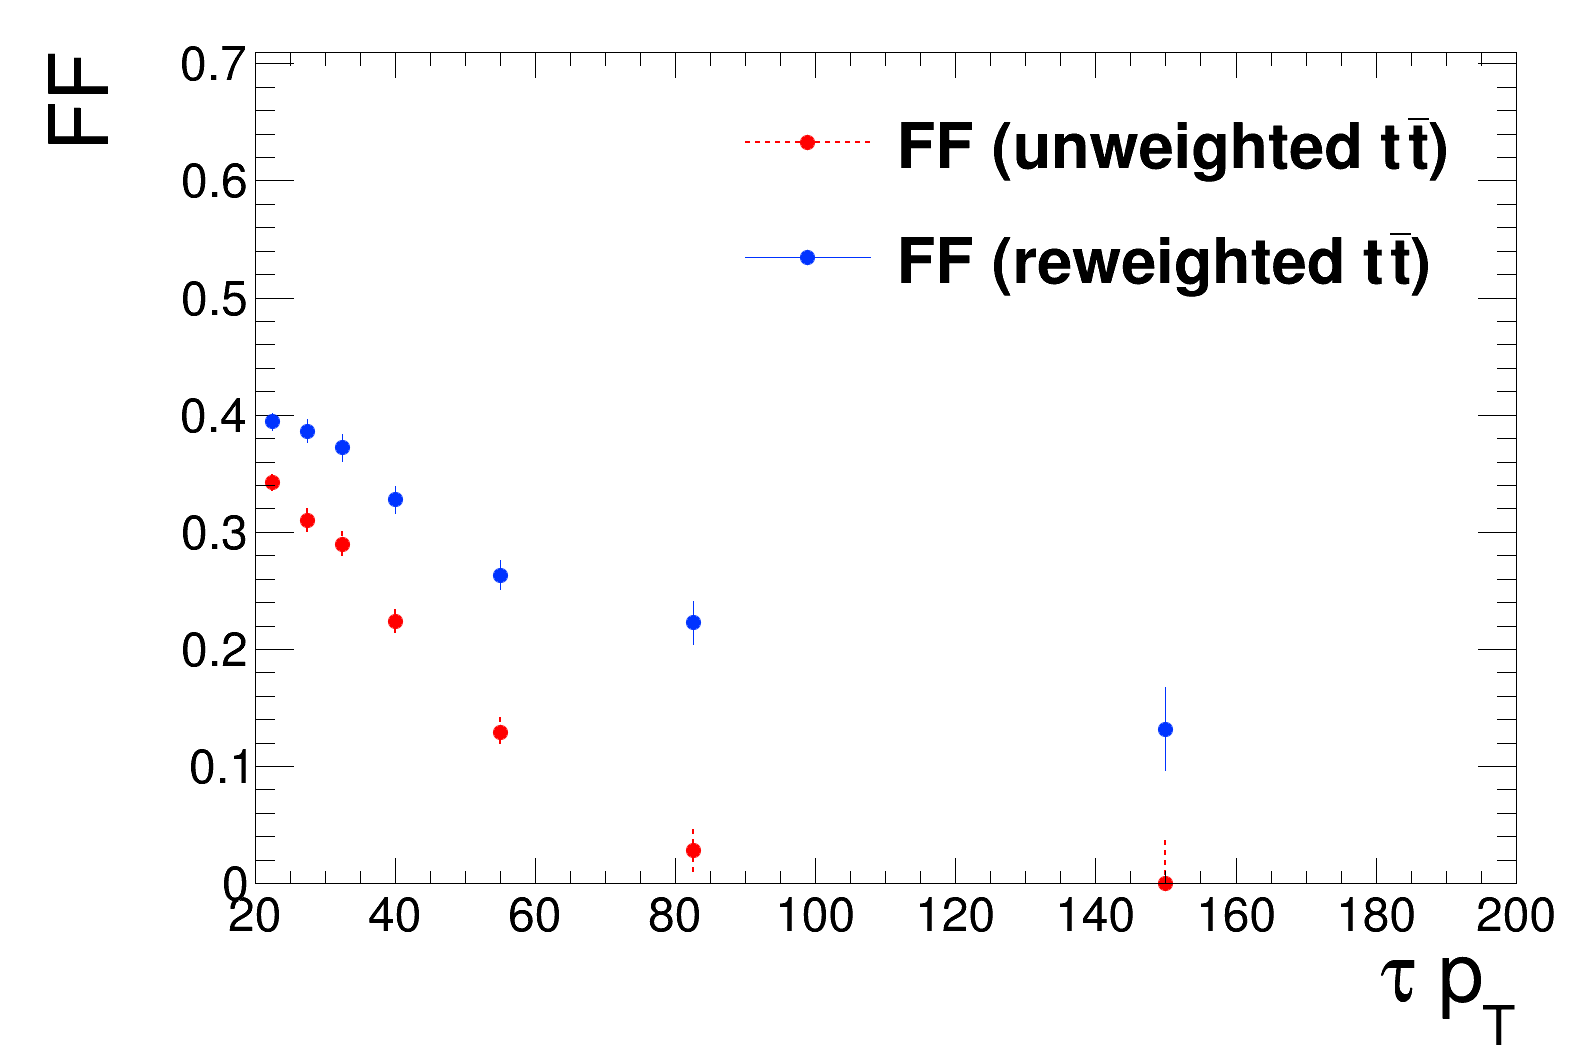
\includegraphics[width=.4\textwidth]{DiHiggs/plots/FF_CRs/SLTttbarCR1p.png}
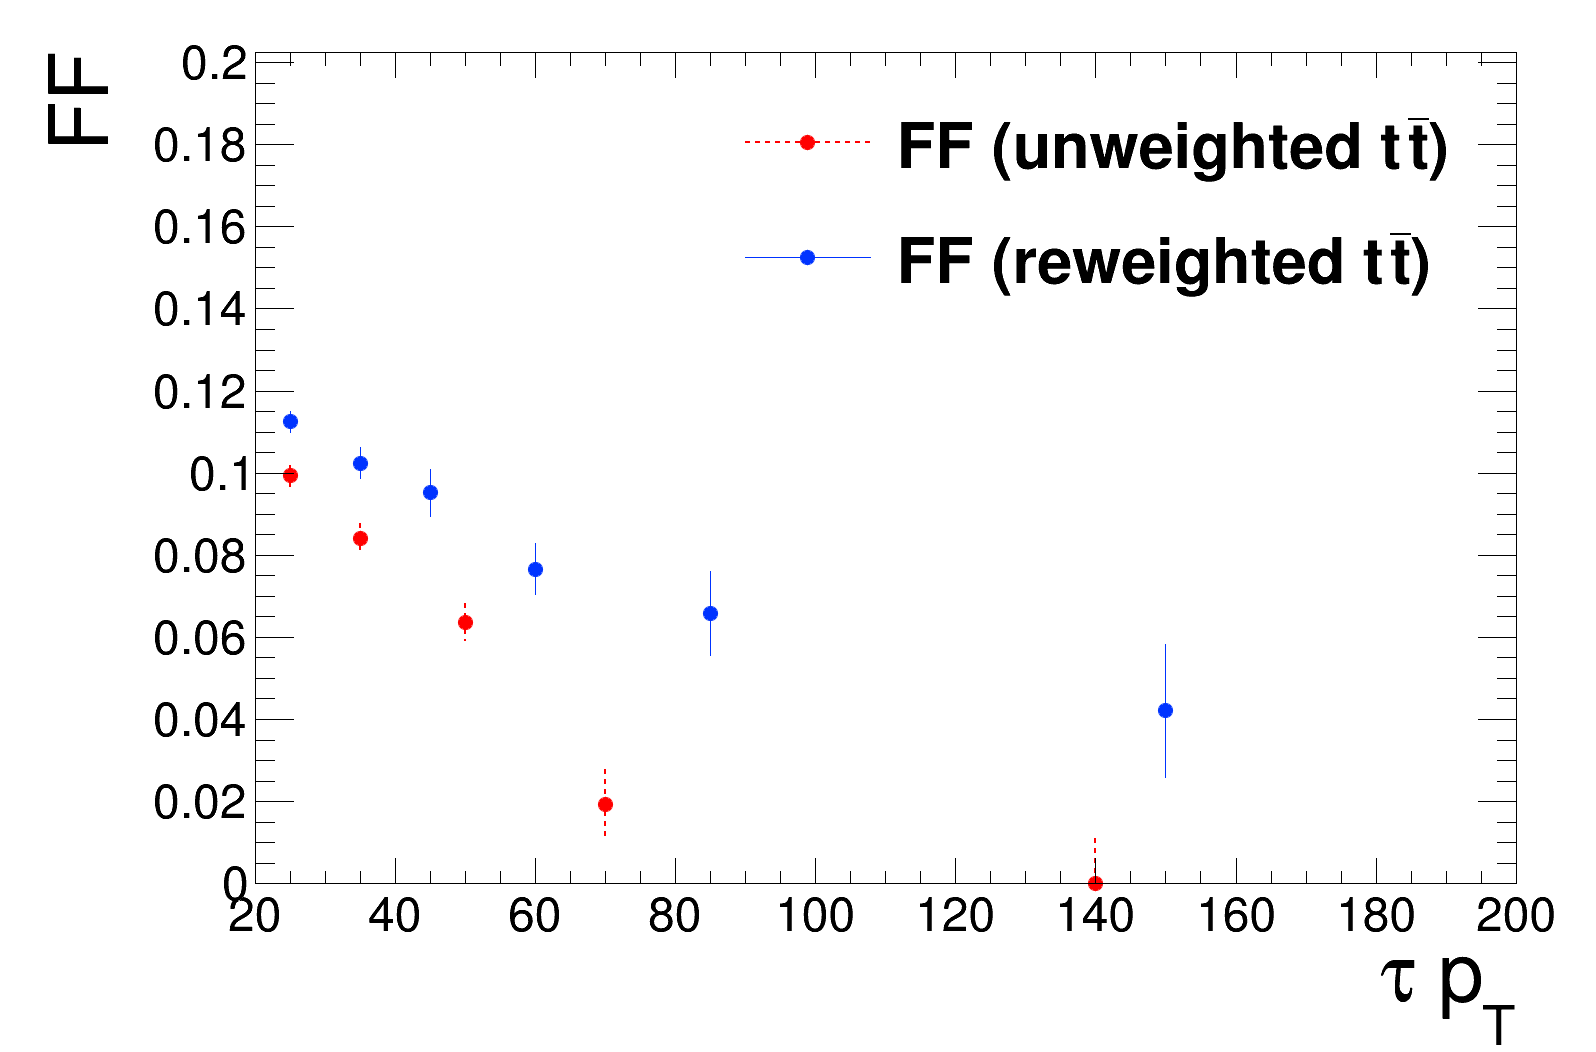
\includegraphics[width=.4\textwidth]{DiHiggs/plots/FF_CRs/SLTttbarCR3p.png} \\
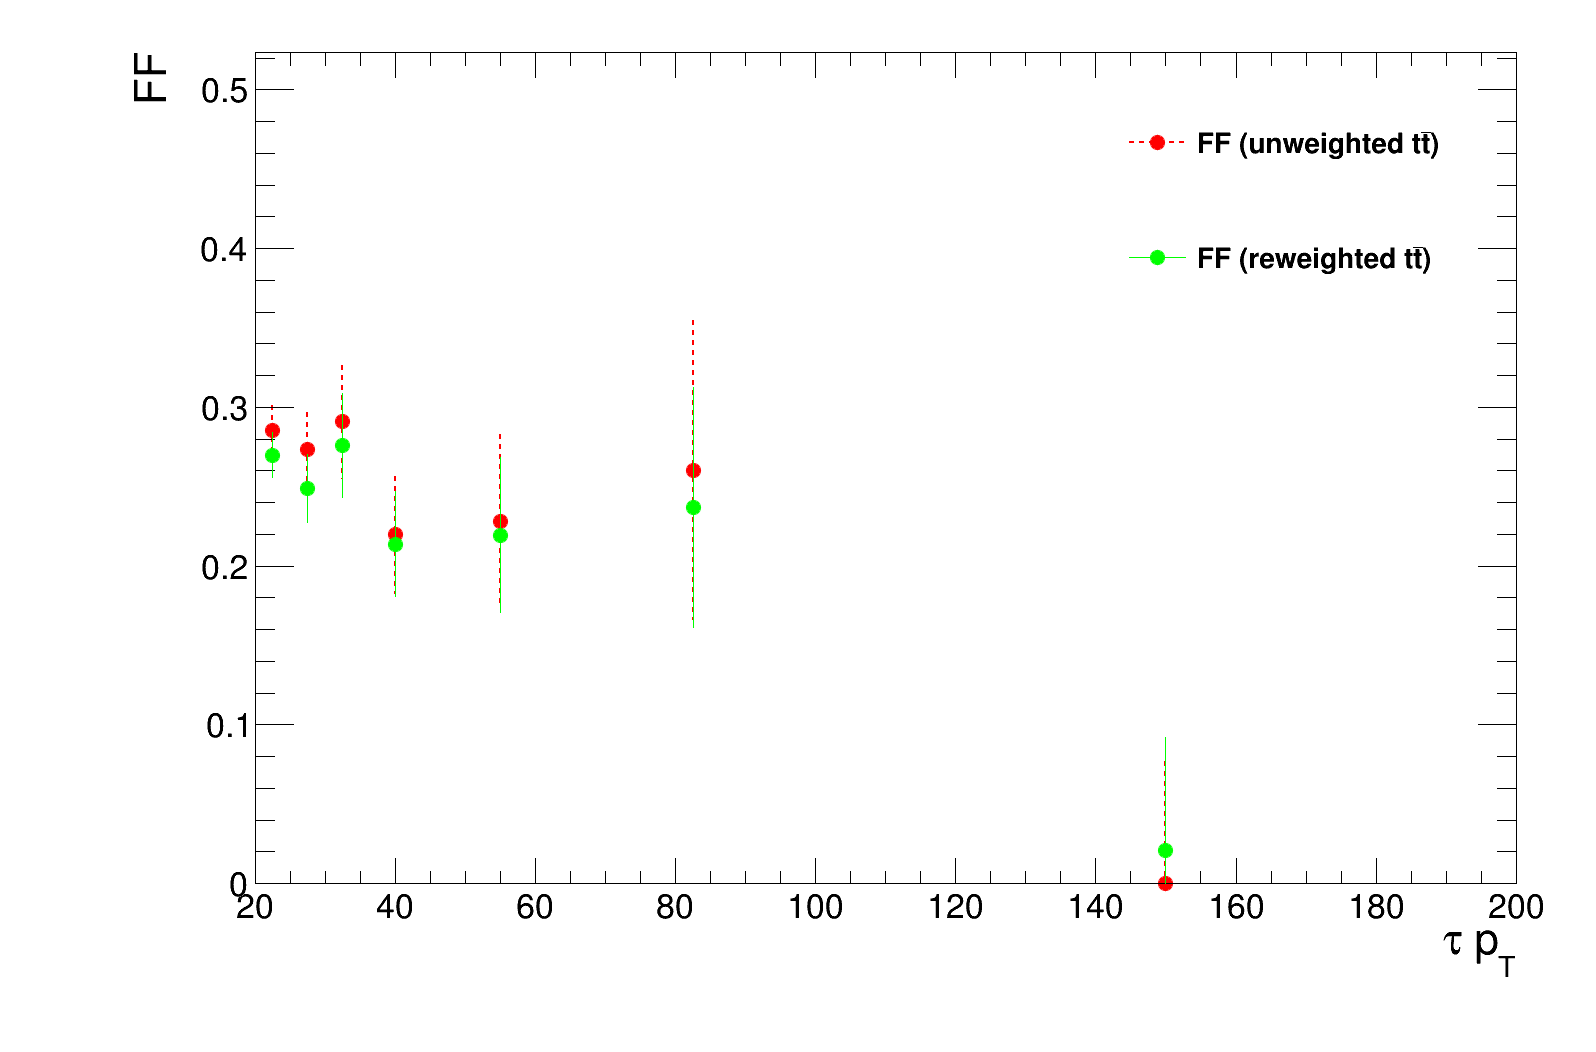
\includegraphics[width=.4\textwidth]{DiHiggs/plots/FF_CRs/SLTInvCR1p.png}
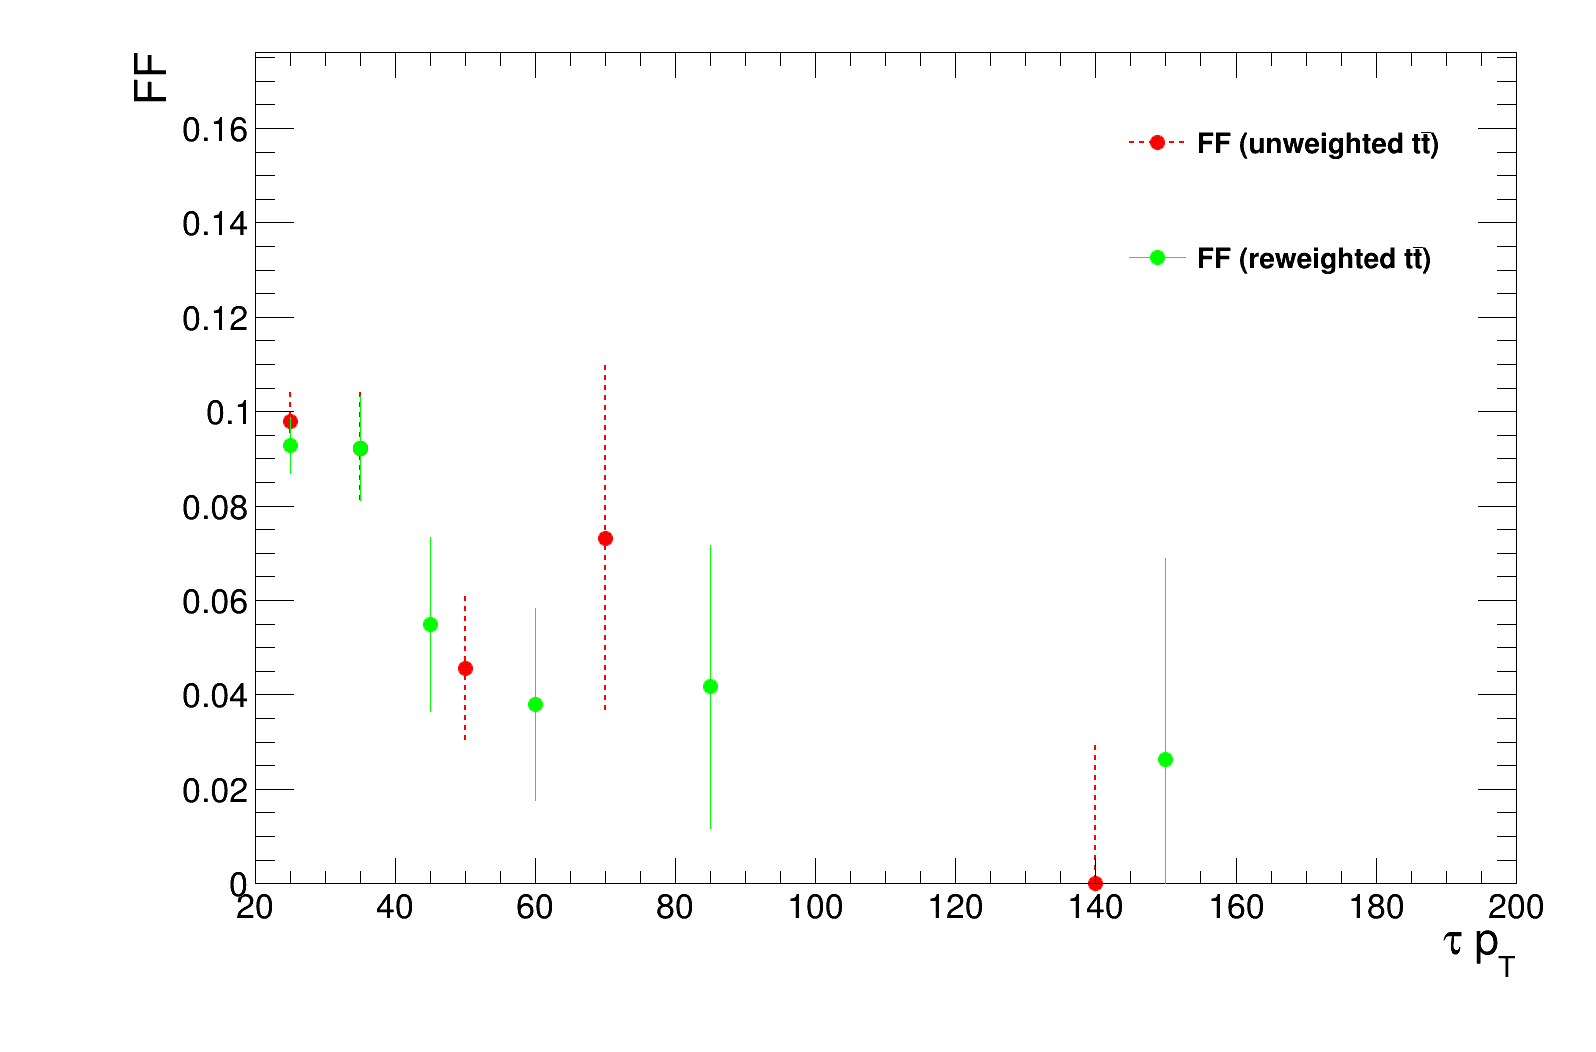
\includegraphics[width=.4\textwidth]{DiHiggs/plots/FF_CRs/SLTInvCR3p.png}\\
\caption{Fake factors 
calculated in \ttbar\ FF-CR (top) and QCD FF-CR (bottom)
for 1-prong (left) and 3-prong (right) 
\tauhad\ candidates for the SLT category.}
\label{fig:SLT_FF}
\end{figure}

\begin{figure}[htbp]
\centering
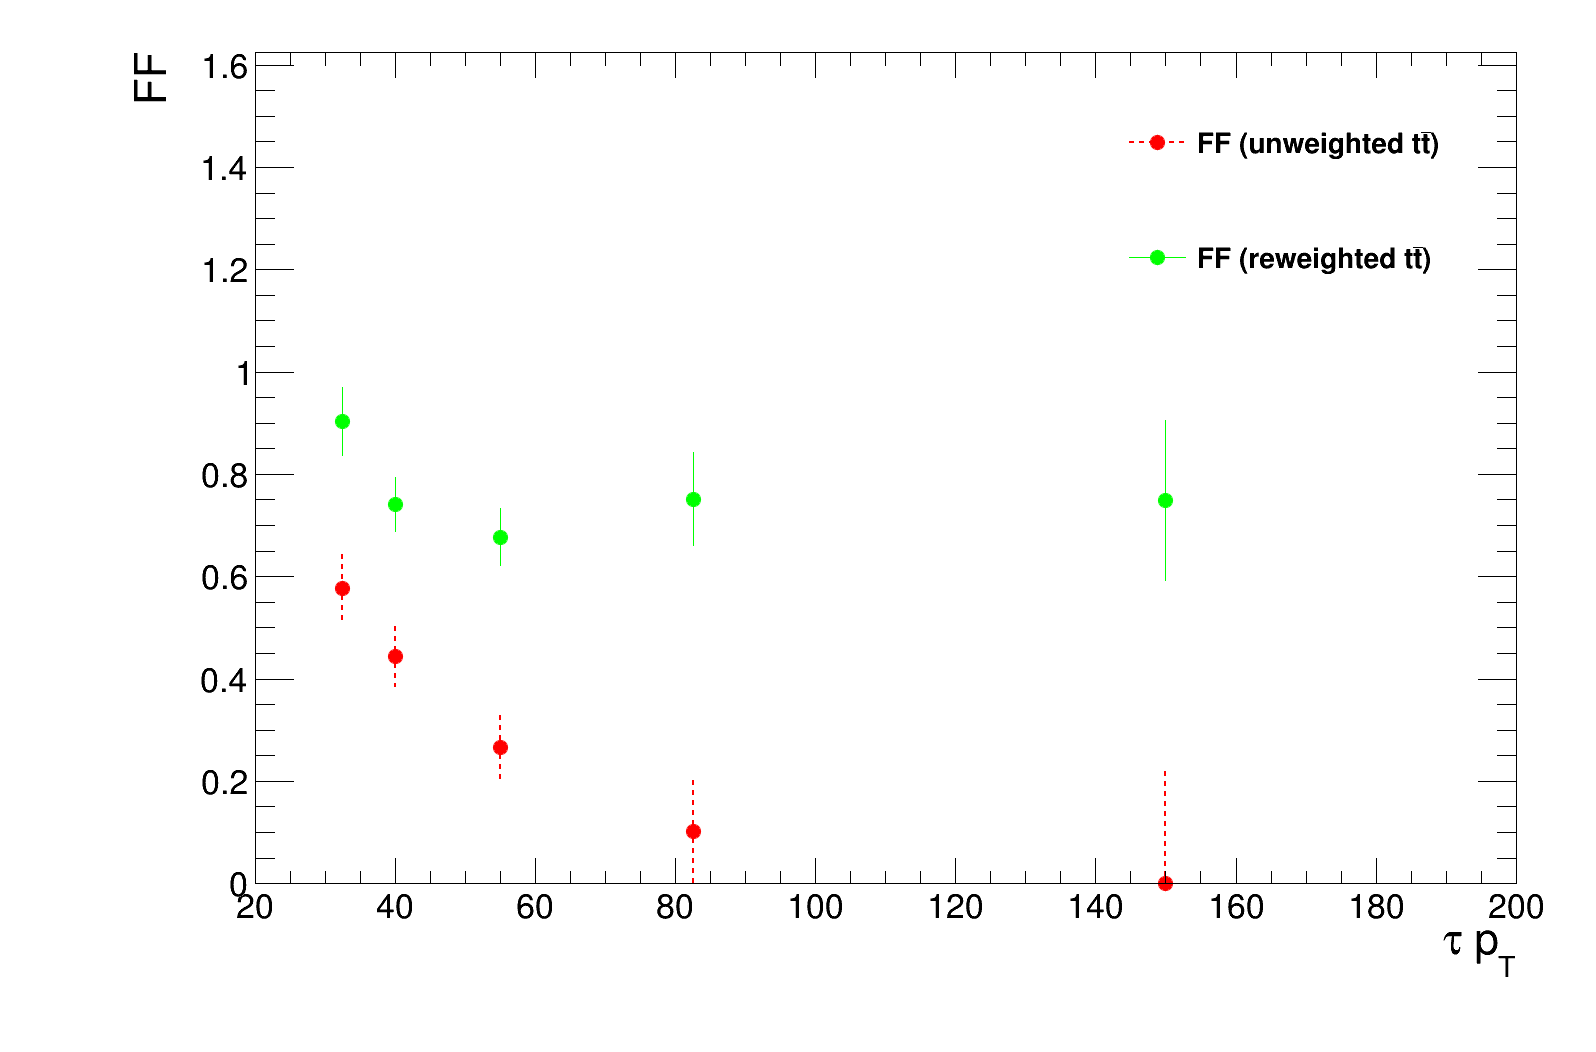
\includegraphics[width=.4\textwidth]{DiHiggs/plots/FF_CRs/LTTttbarCR1p.png}
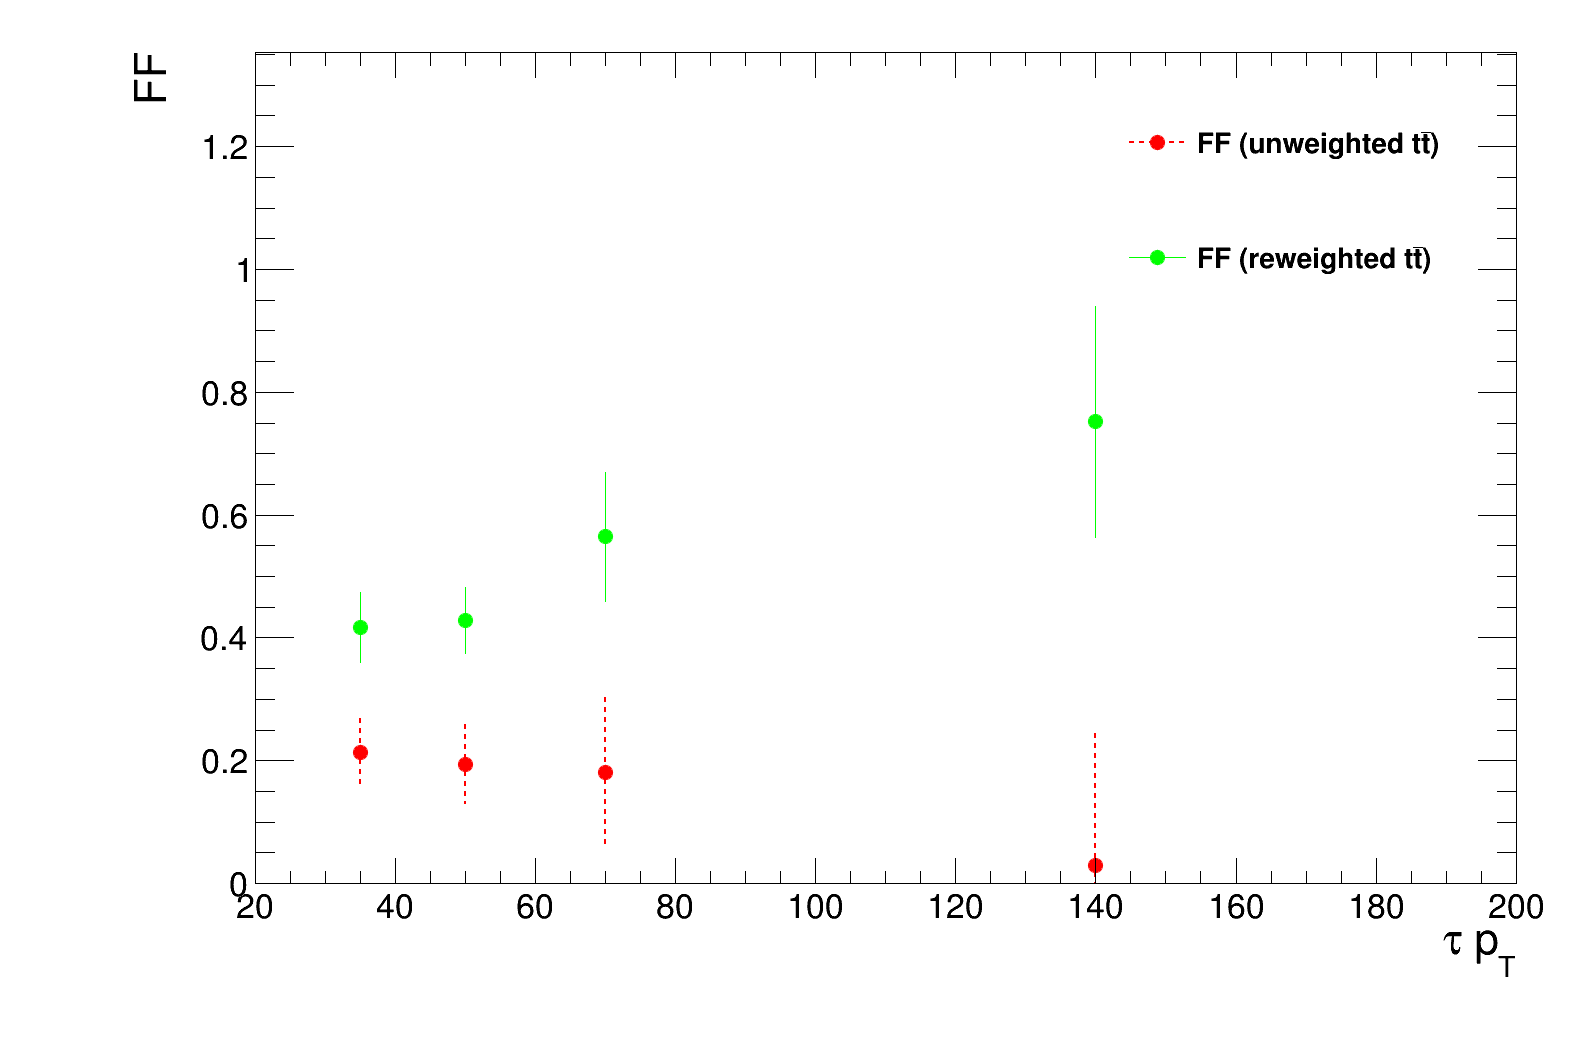
\includegraphics[width=.4\textwidth]{DiHiggs/plots/FF_CRs/LTTttbarCR3p.png} \\
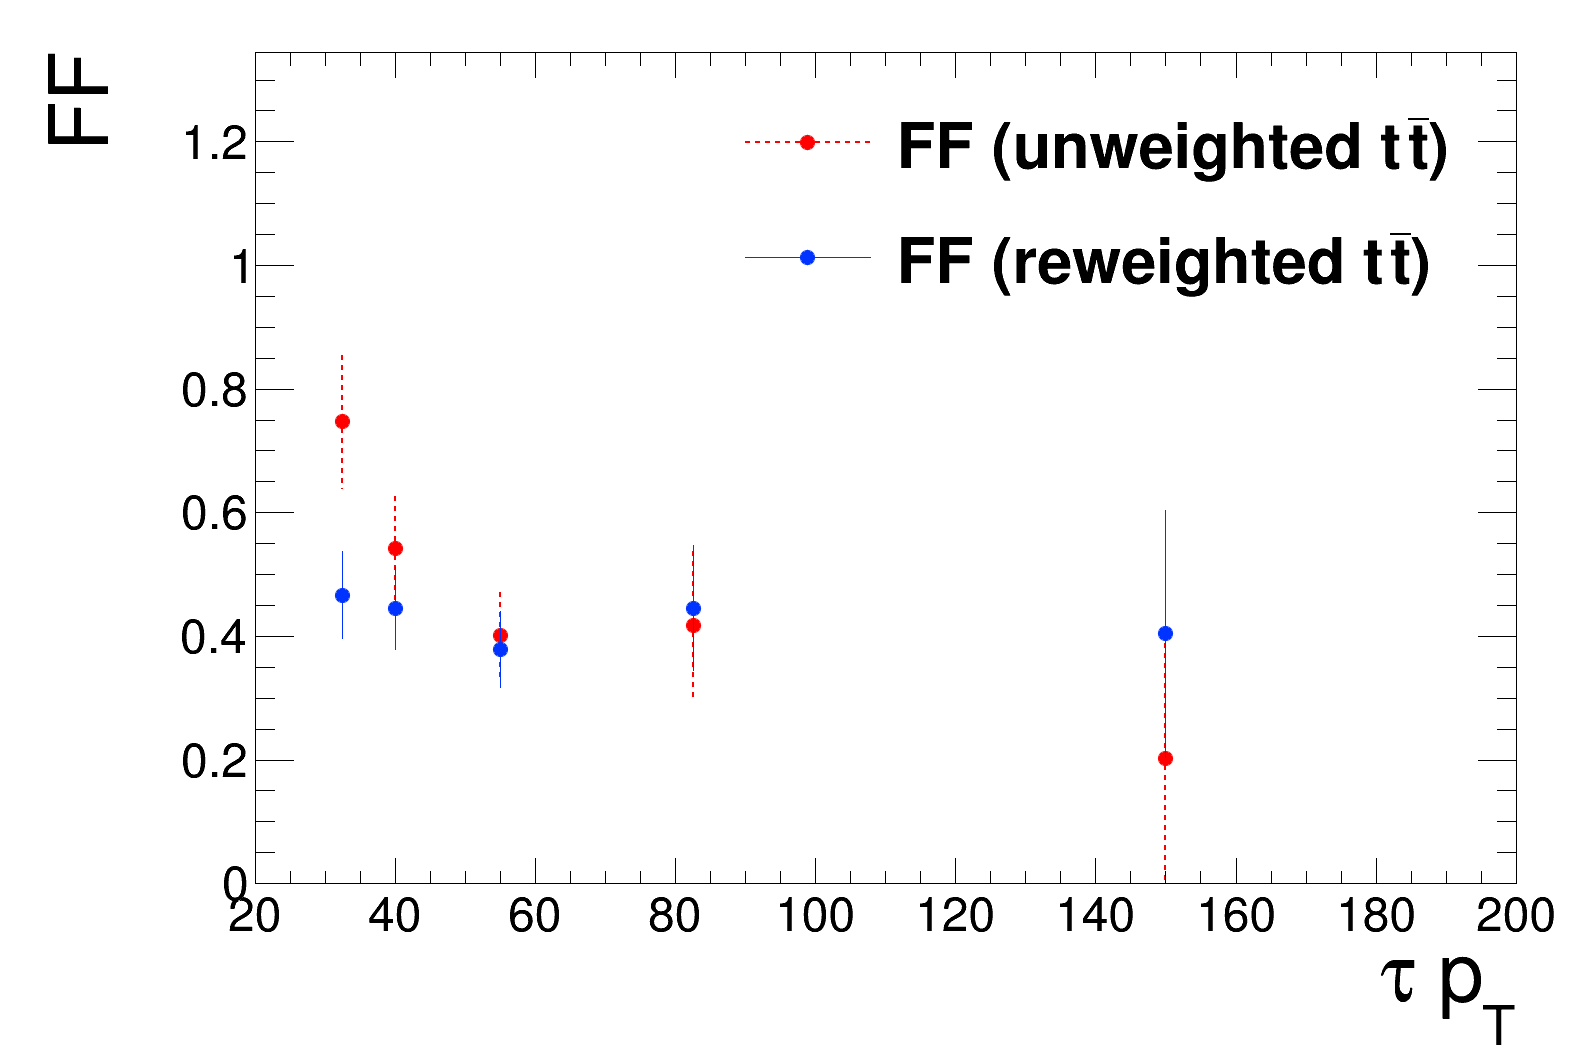
\includegraphics[width=.4\textwidth]{DiHiggs/plots/FF_CRs/LTTInvCR1p.png}
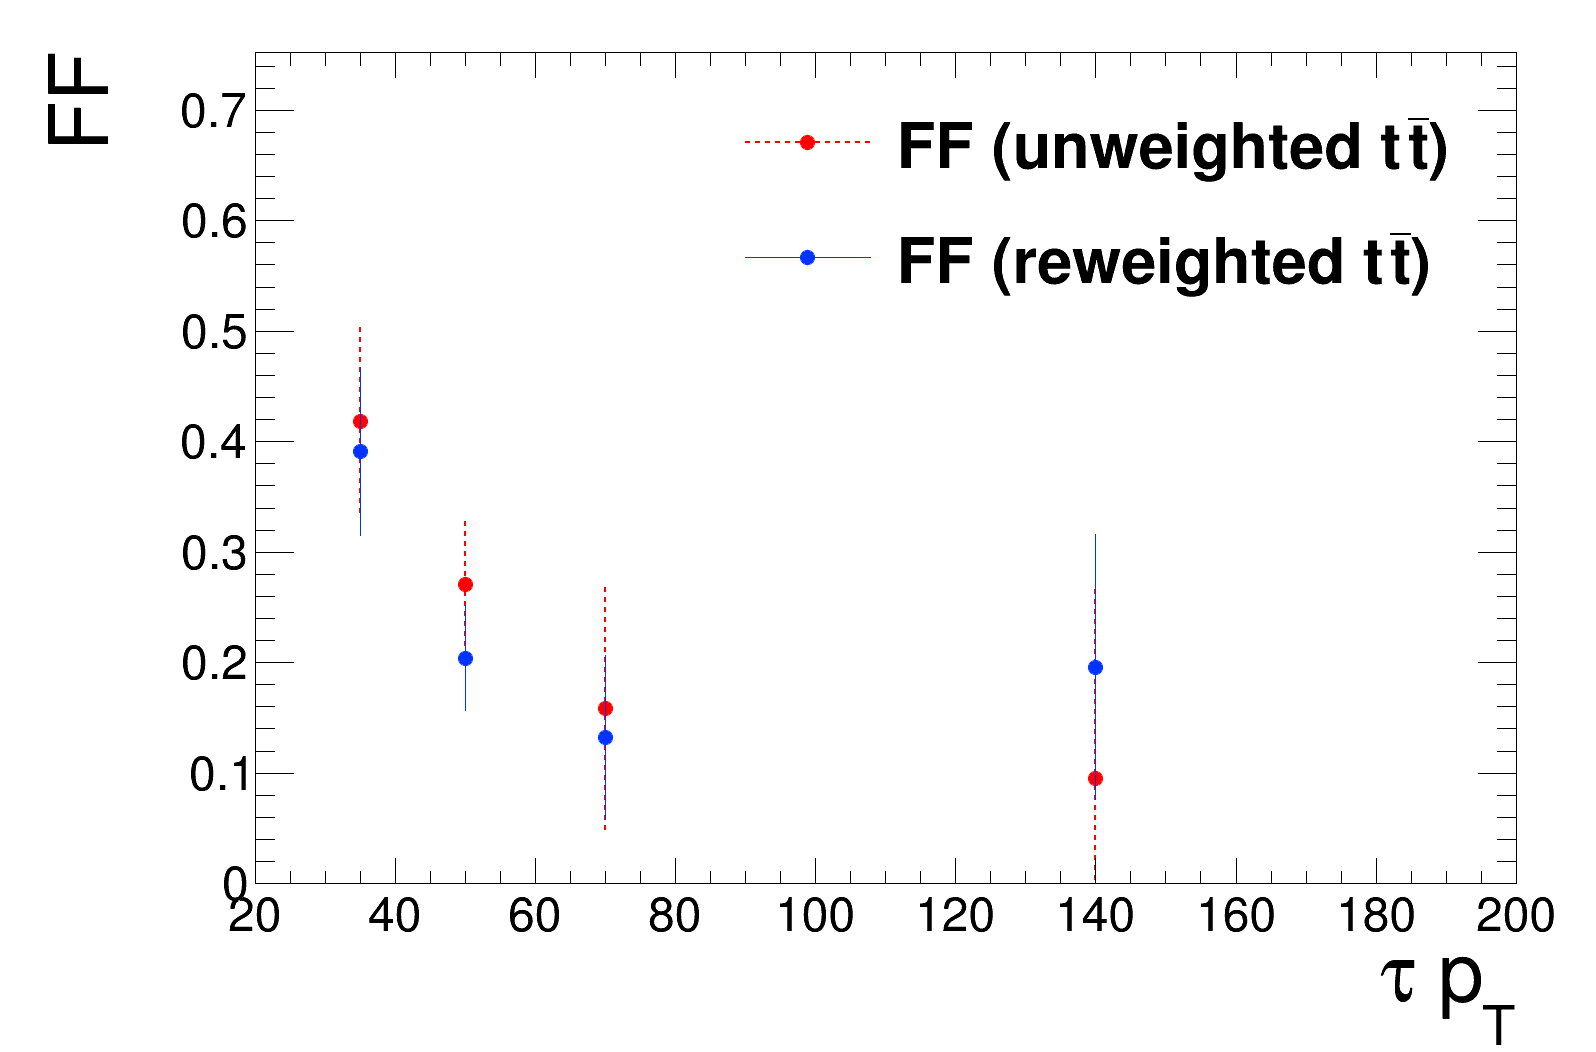
\includegraphics[width=.4\textwidth]{DiHiggs/plots/FF_CRs/LTTInvCR3p.png}\\
\caption{Fake factors 
calculated in \ttbar\ FF-CR (top) and QCD FF-CR (bottom)
for 1-prong (left) and 3-prong (right) 
\tauhad\ candidates for the LTT category.}
\label{fig:LTT_FF}
\end{figure}

\begin{figure}[htbp]
\centering
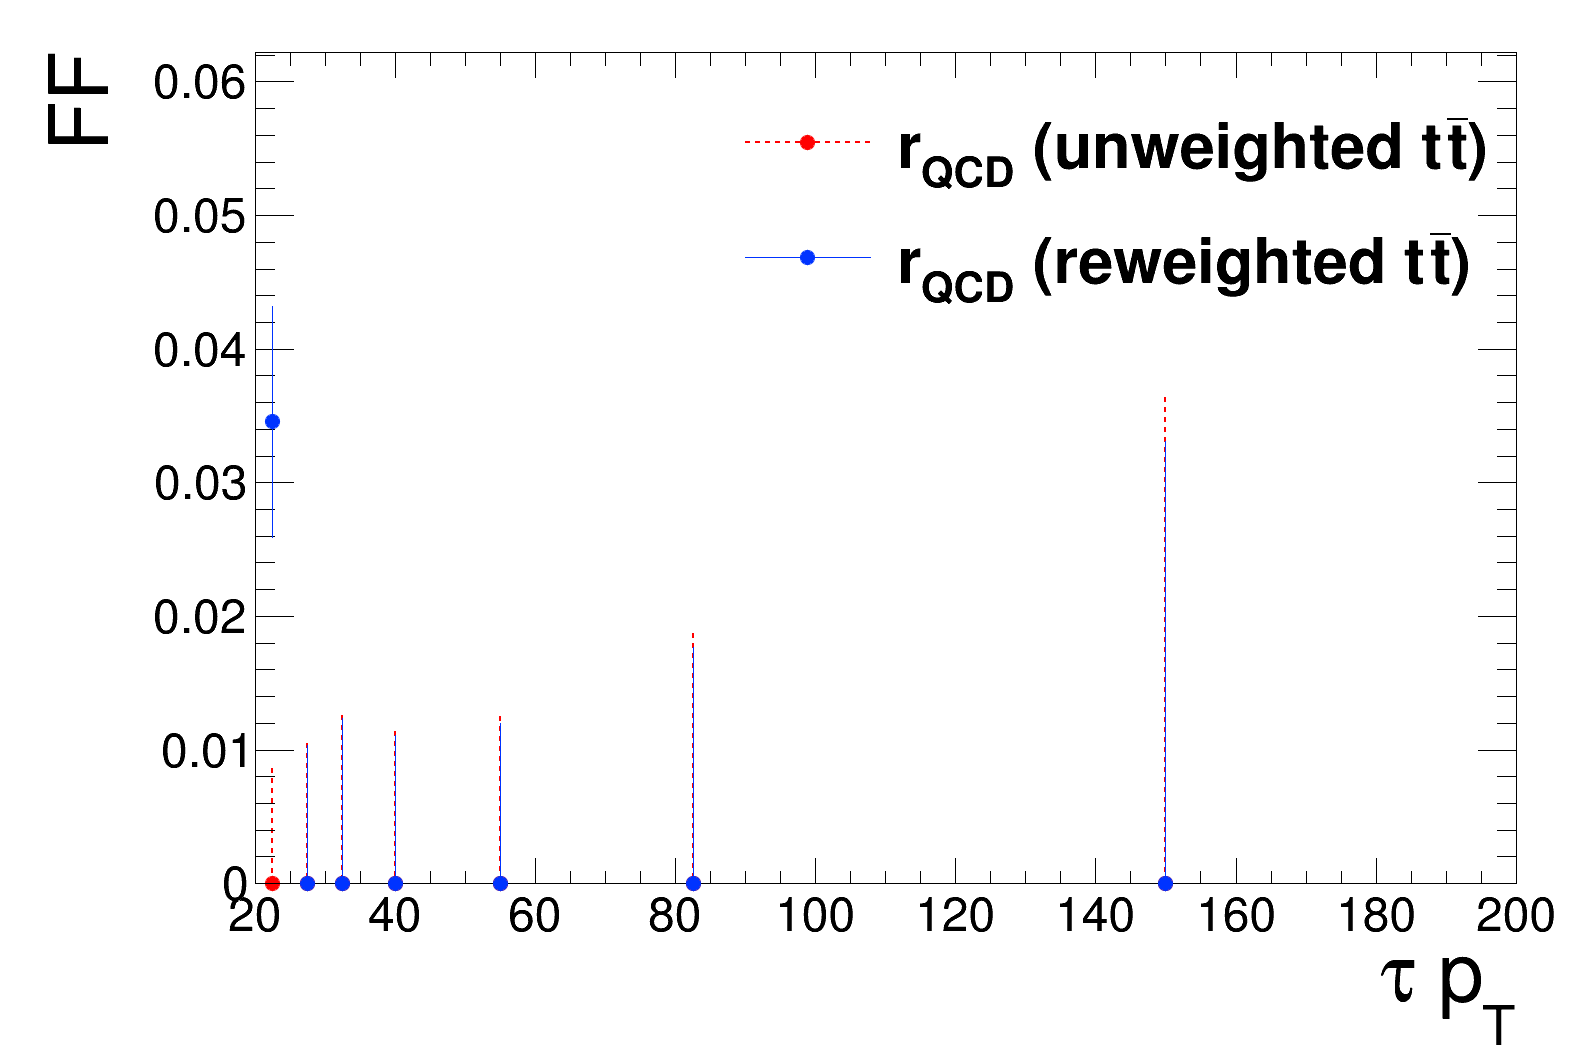
\includegraphics[width=.4\textwidth]{DiHiggs/plots/FF_CRs/SLTElecrQCD1p.png}
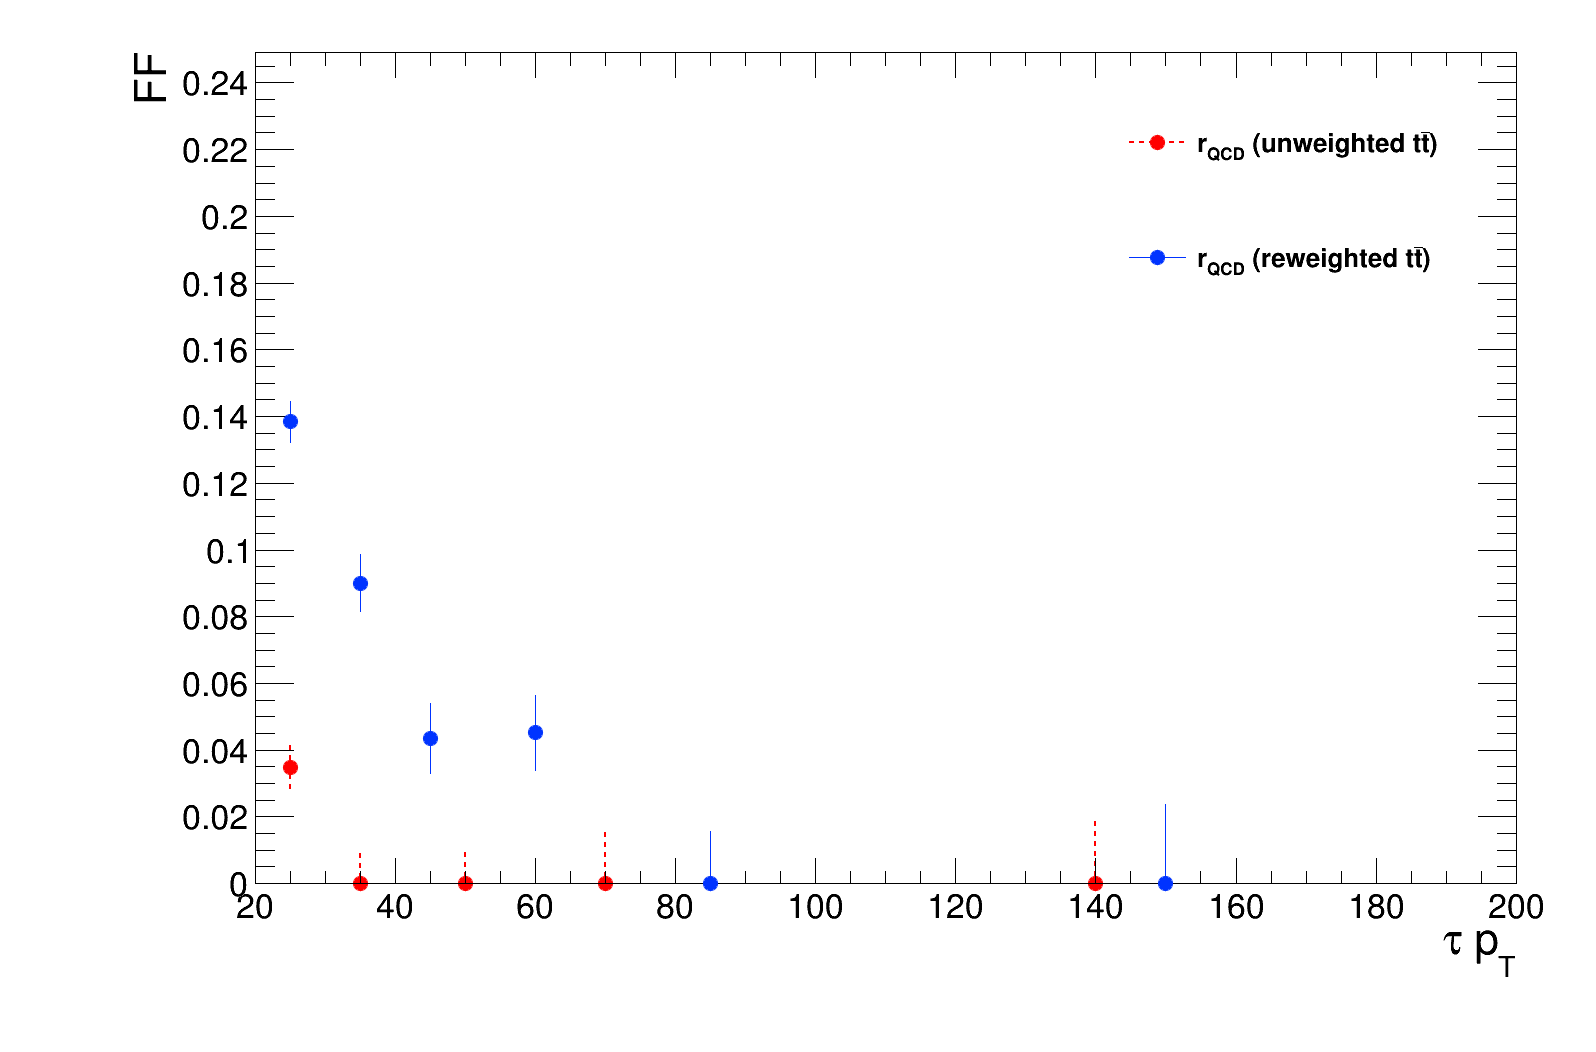
\includegraphics[width=.4\textwidth]{DiHiggs/plots/FF_CRs/SLTElecrQCD3p.png} \\
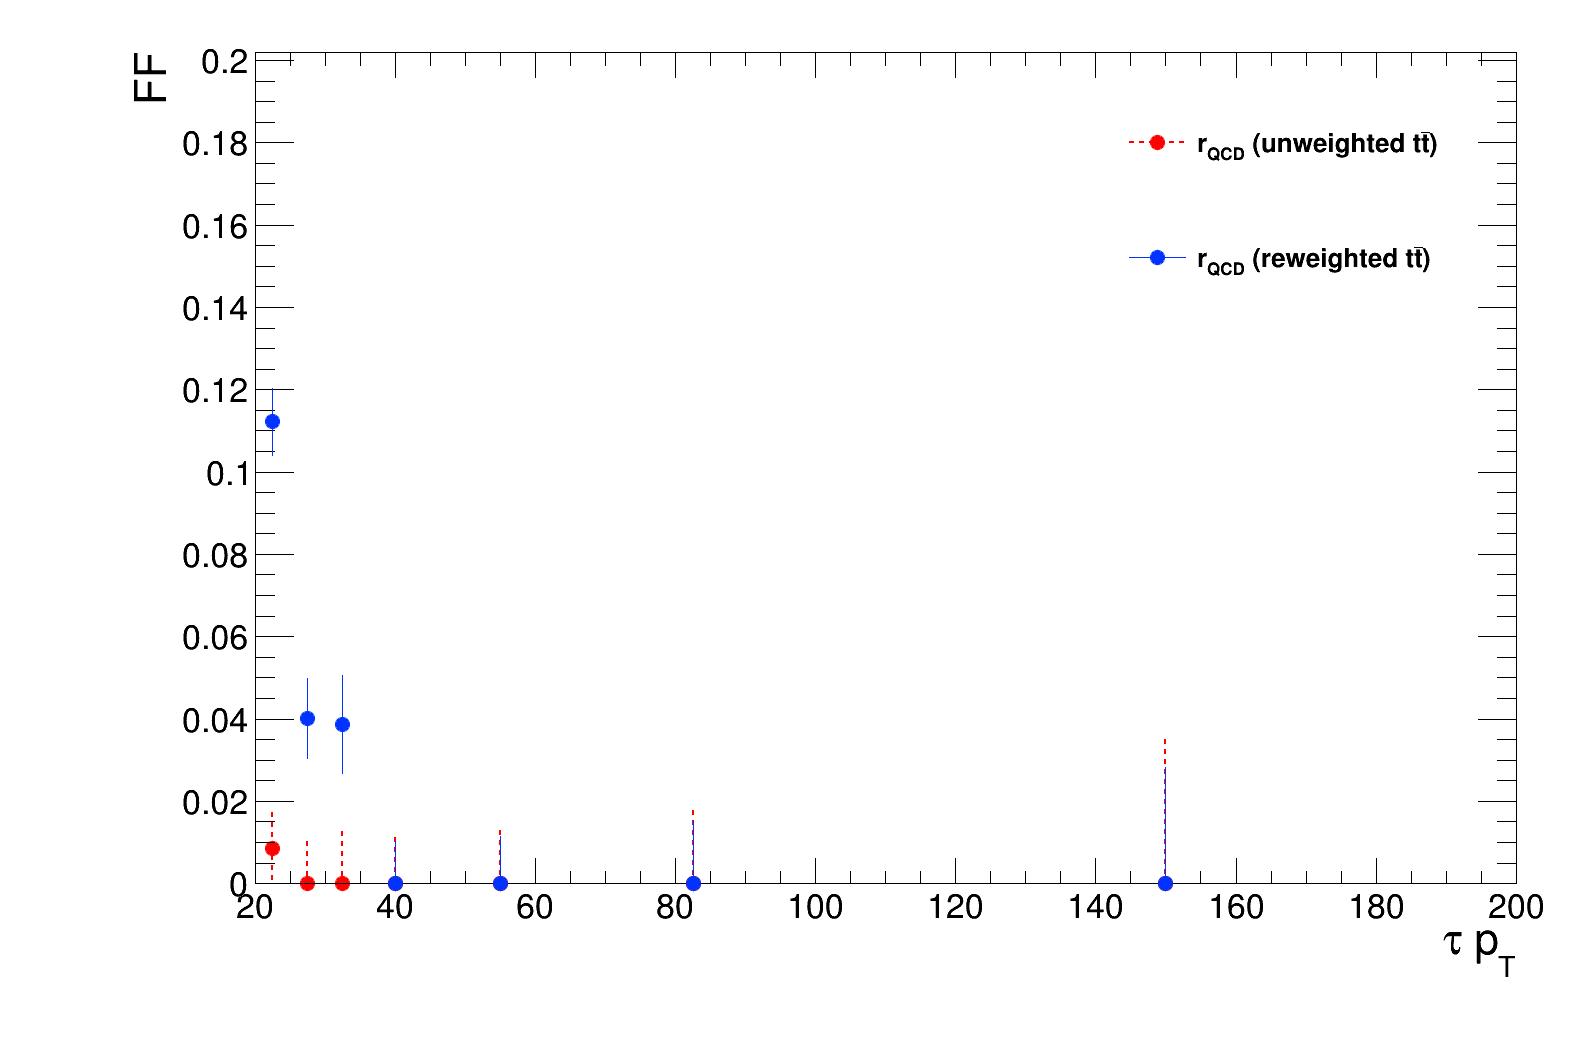
\includegraphics[width=.4\textwidth]{DiHiggs/plots/FF_CRs/SLTMuonrQCD1p.png}
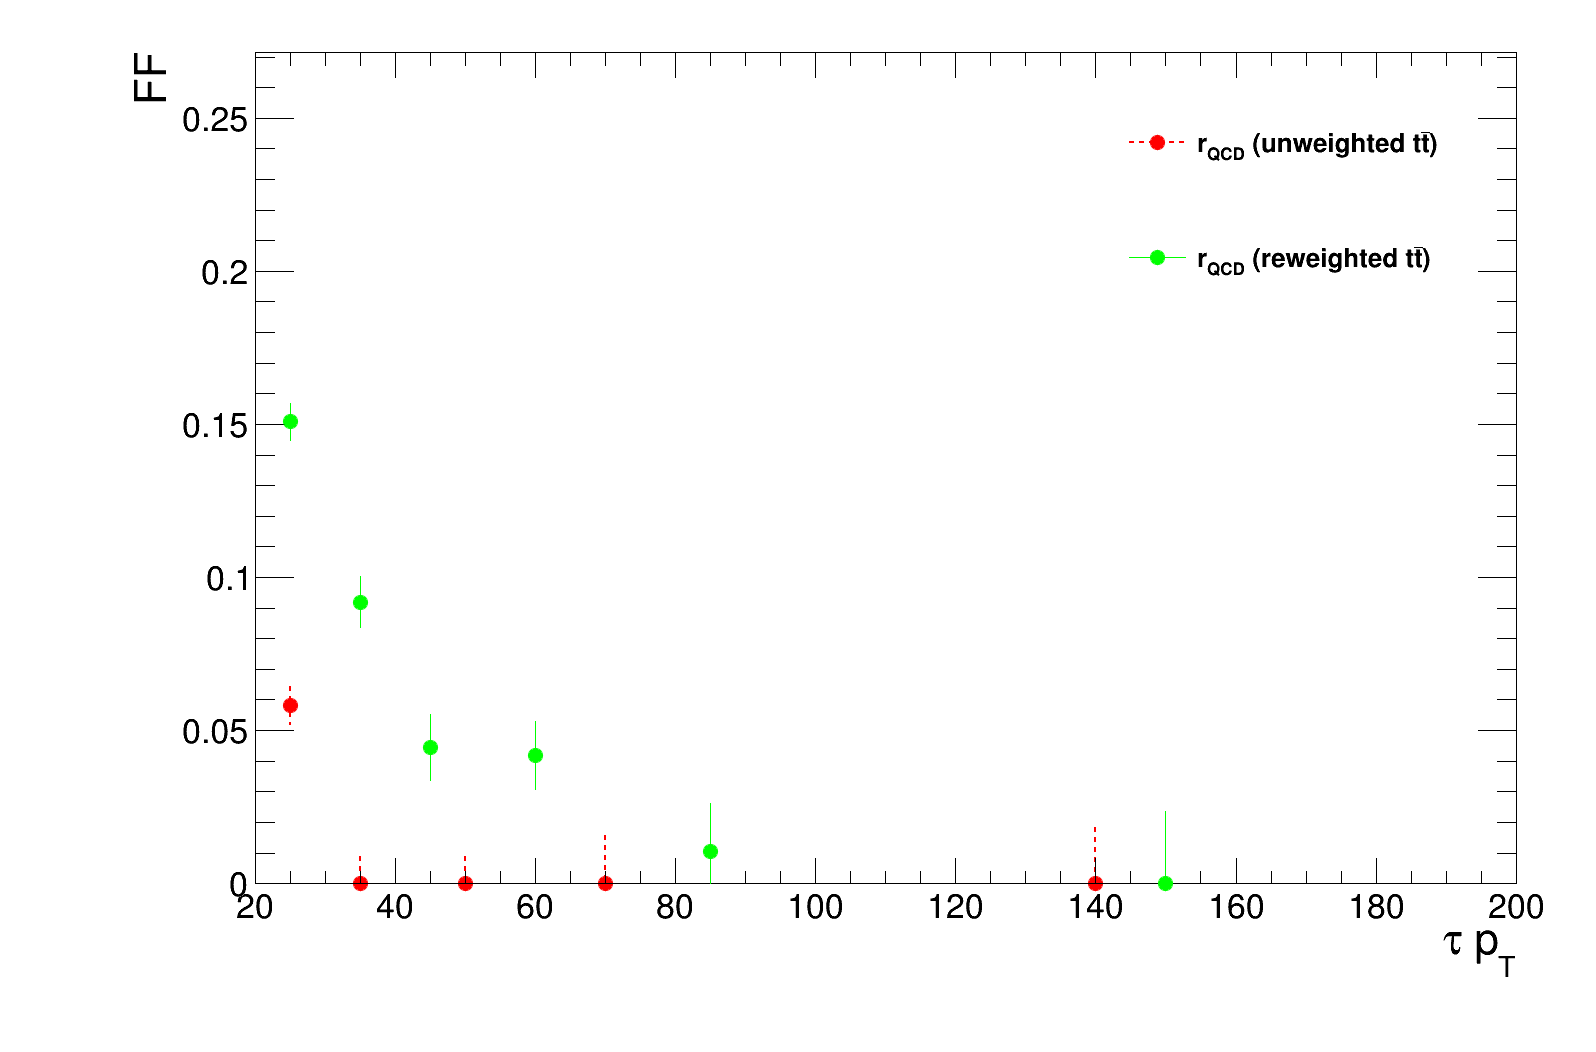
\includegraphics[width=.4\textwidth]{DiHiggs/plots/FF_CRs/SLTMuonrQCD3p.png}\\
\caption{$\mathrm{r}_{\mathrm{QCD}}$ for 1-prong (left) 
and 3-prong (right) \tauhad\ candidates with $e\tauhad$ 
 (top) and $\mu\tauhad$ (bottom) final states
for the SLT channel.}
\label{fig:SLT_rQCD}
\end{figure}

\begin{figure}[htbp]
\centering
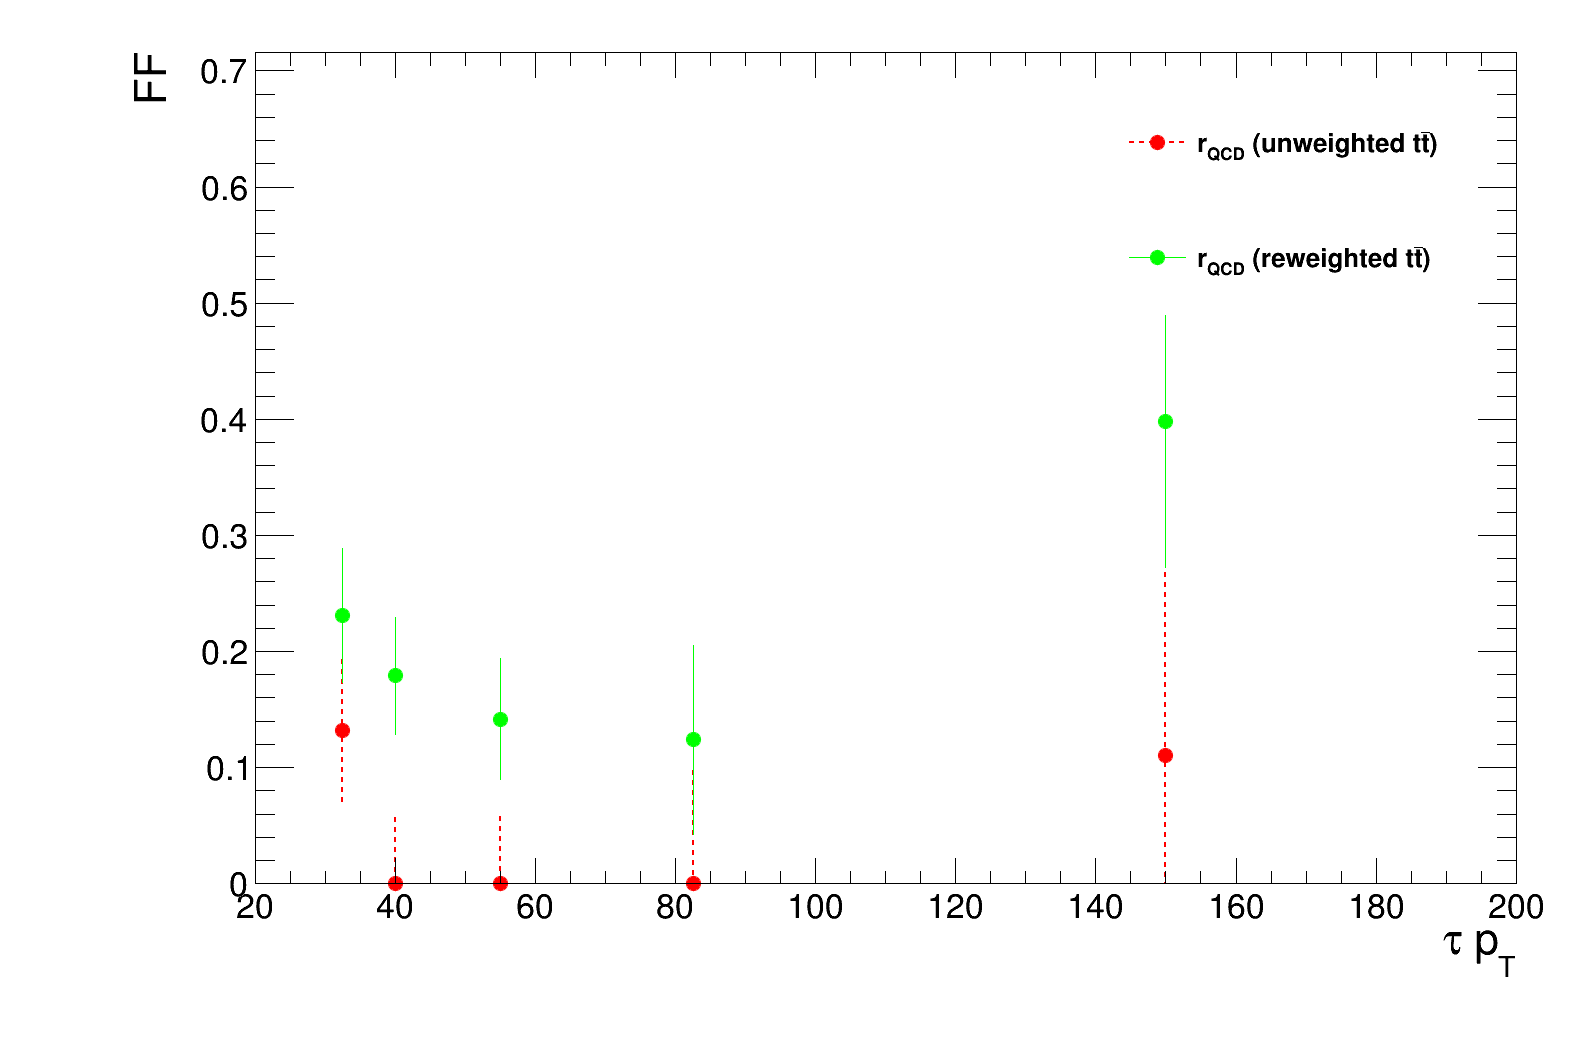
\includegraphics[width=.4\textwidth]{DiHiggs/plots/FF_CRs/LTTElecrQCD1p.png}
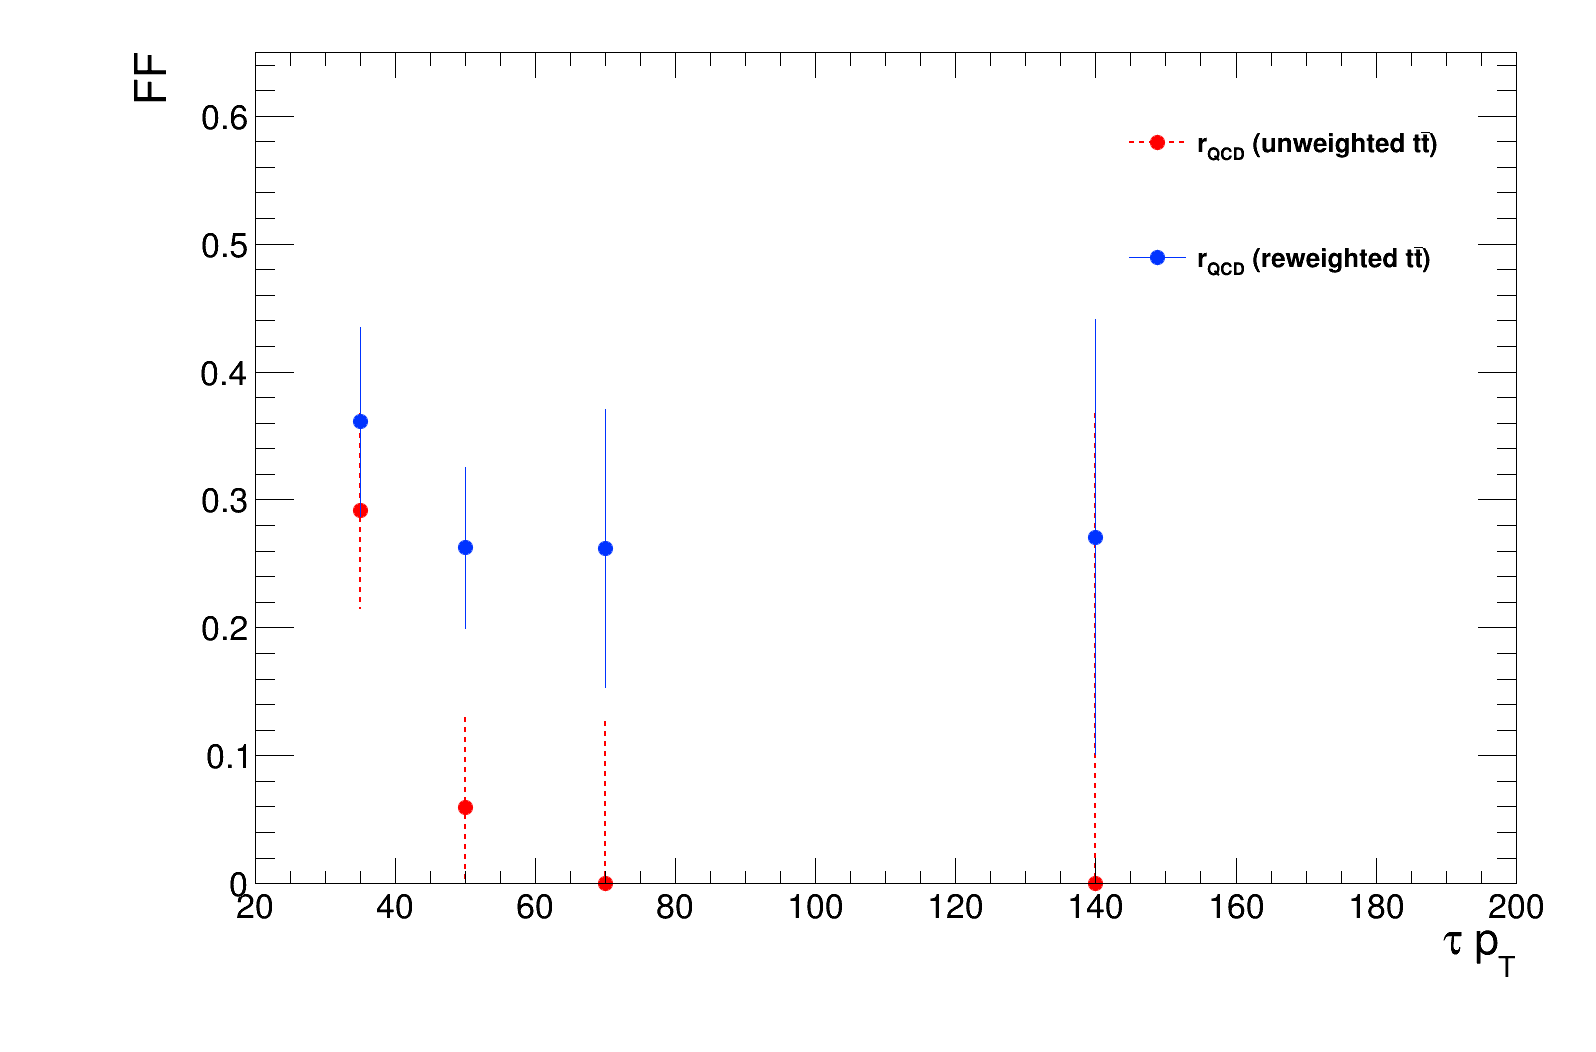
\includegraphics[width=.4\textwidth]{DiHiggs/plots/FF_CRs/LTTElecrQCD3p.png} \\
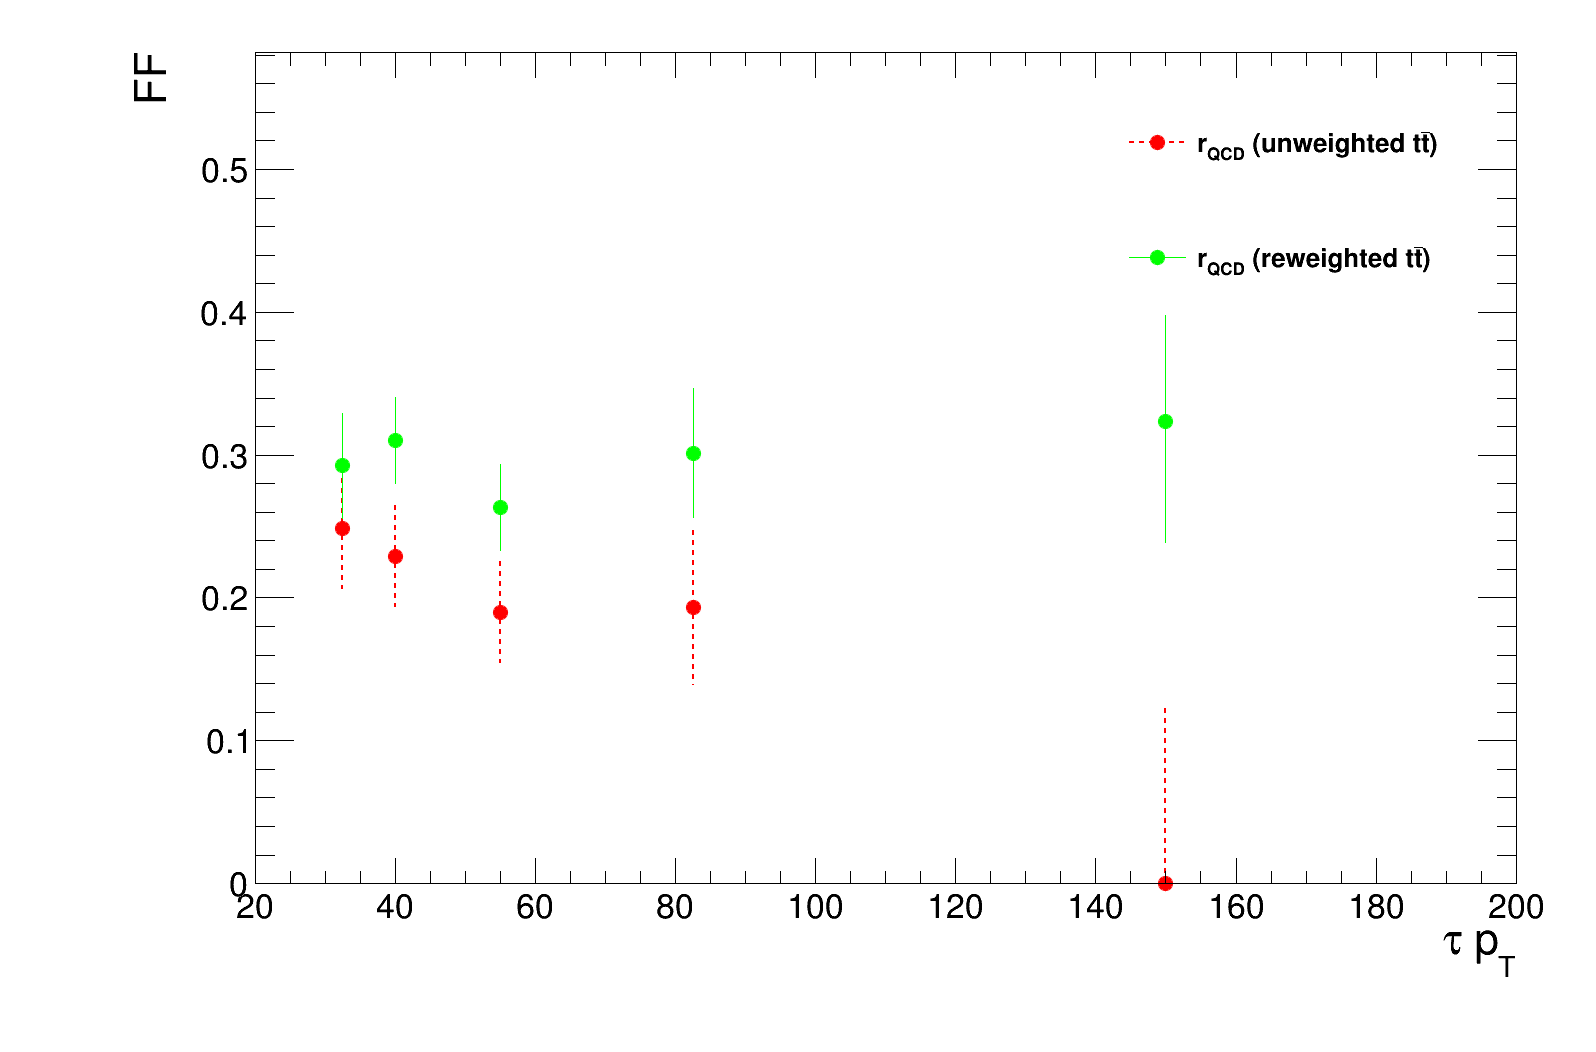
\includegraphics[width=.4\textwidth]{DiHiggs/plots/FF_CRs/LTTMuonrQCD1p.png}
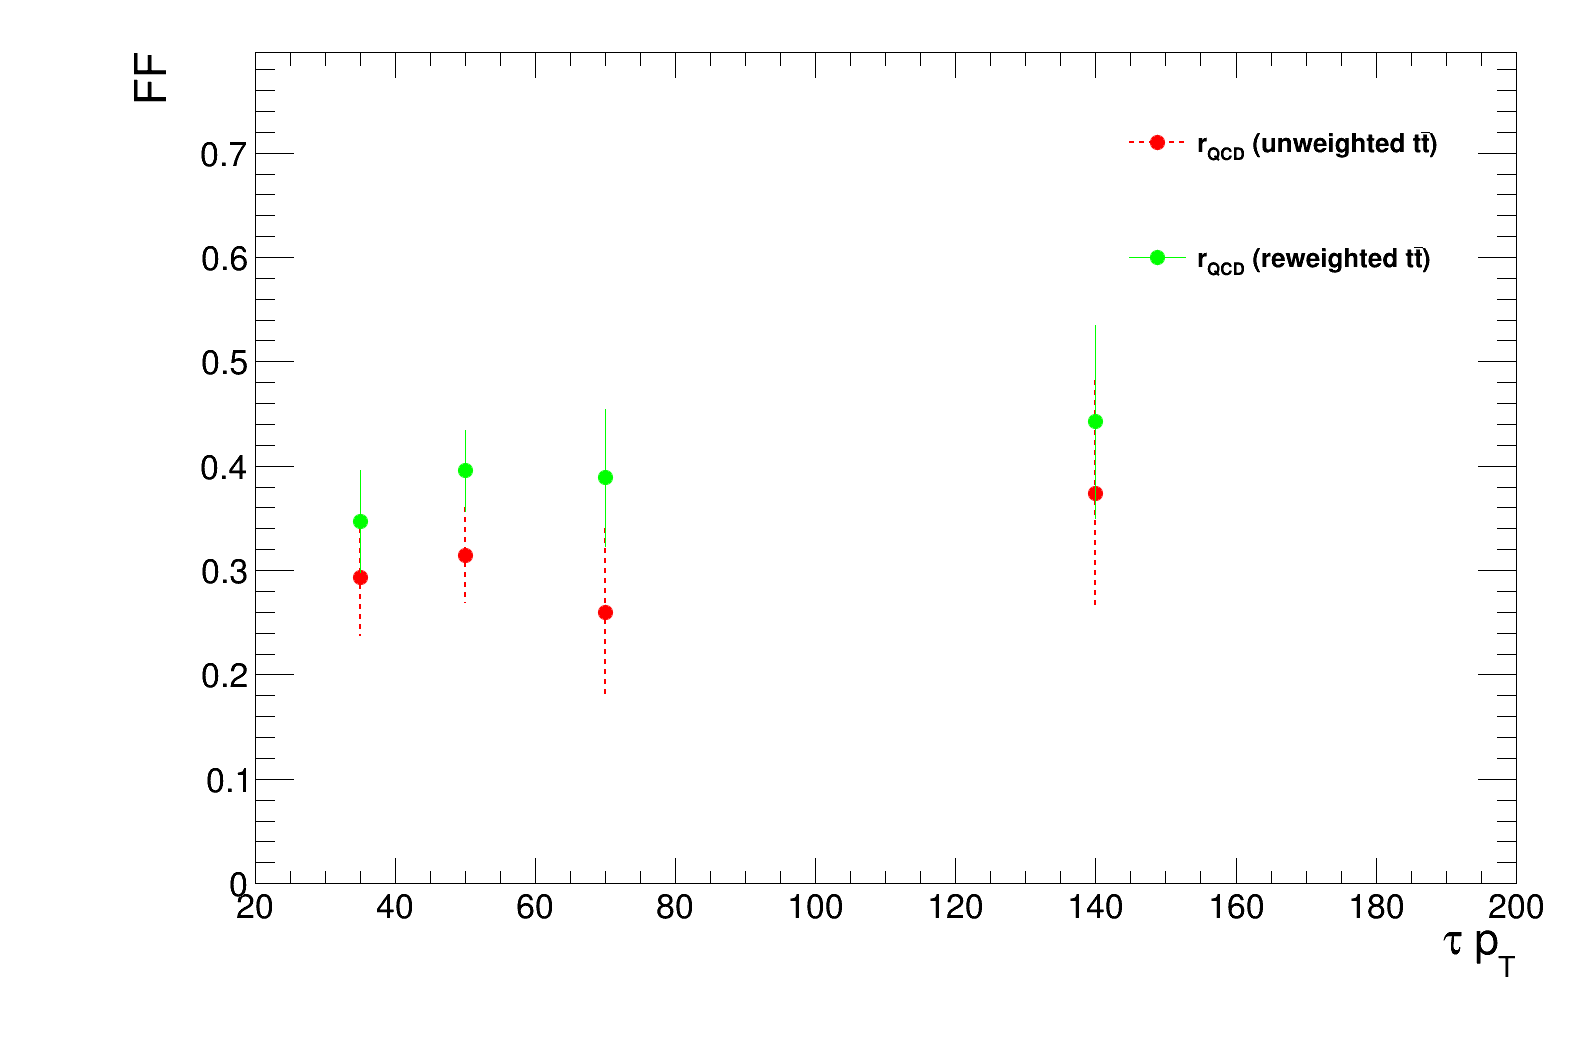
\includegraphics[width=.4\textwidth]{DiHiggs/plots/FF_CRs/LTTMuonrQCD3p.png}\\
\caption{$\mathrm{r}_{\mathrm{QCD}}$ for 1-prong (left) 
and 3-prong (right) \tauhad\ candidates with $e\tauhad$ 
 (top) and $\mu\tauhad$ (bottom) final states
for the LTT channel.}
\label{fig:LTT_rQCD}
\end{figure}
%%%
% The difference between the fake-\tauhad\ background estimations obtained with and without
% the aforementioned $t\bar{t}$ modelling correction is taken as an uncertainty in the background estimate.
% A conservative 30\% modelling uncertainty is assigned to simulated non-$t\bar t$ backgrounds
% which are subtracted from data.
%%%The value of $\mathrm{r}_\text{multi-jet}$ is allowed to vary within $\pm 0.5$ with respect to the nominal estimate
%%%in the signal extraction fit to account for uncertainties in the modelling of the simulation used in its calculation.
% Due to its large dependence on the modelling of simulated $t\bar{t}$ events with fake-\tauhad\ 
% the obtained values of $\mathrm{r}_\text{multi-jet}$ are varied by $\pm 0.5$, while enforcing $0\leq r_\text{QCD}\leq 1$. 
% The impact of such a conservative uncertainty is small since the FFs in multi-jet and $t\bar{t}$ events are found to be similar.
%%%
% The total uncertainty on the $\text{FF}_\text{comb}$ for the SLT category is up to 10\% and
% up to 25\% for the LTT category.
%%%
Statistical uncertainties in $\text{FF}_{t\bar{t}}$, $\text{FF}_\text{QCD}$ and $\mathrm{r}_\text{QCD}$
are evaluated and propagated to the final result,
and a conservative 30\% modelling uncertainty is assigned to simulated non-$t\bar t$ backgrounds
which are subtracted from data.
The uncertainties due to \ttbar\ modelling issue and its subtraction are discussed in more details
in section~\ref{sec:DiHiggs:fakesysts}.TODO: add reference to the systematics section.

\subsubsection{Fake factor method validation}
The combined FF method is validated in
the 0-$b$-tagged and 1-$b$-tagged regions, where the same event selection as SR 
is applied but with different numbers of $b$-tagged jets required. 
The fakes in each validation region are estimated with FF calculated in each validation region 
with the same method used in the 2-$b$-tagged region.
These two validation regions are chosen as 
the signal contamination in the 0-$b$-tagged 
and 1-$b$-tagged regions is negligible,
and the 0-$b$-tagged region can benefit from its rich statistics 
and the 1-$b$-tagged region can benefit from being closer to the SR.
The estimated background distributions agree well 
with the observed distributions in all validation regions.
The data and MC comparison with fakes estimated with the FF method 
are shown in Figure~\ref{fig:FFVRSLT} for the SLT channel and
Figure~\ref{fig:FFVRLTT} for the LTT channel. 

\begin{figure}[htbp]
\centering
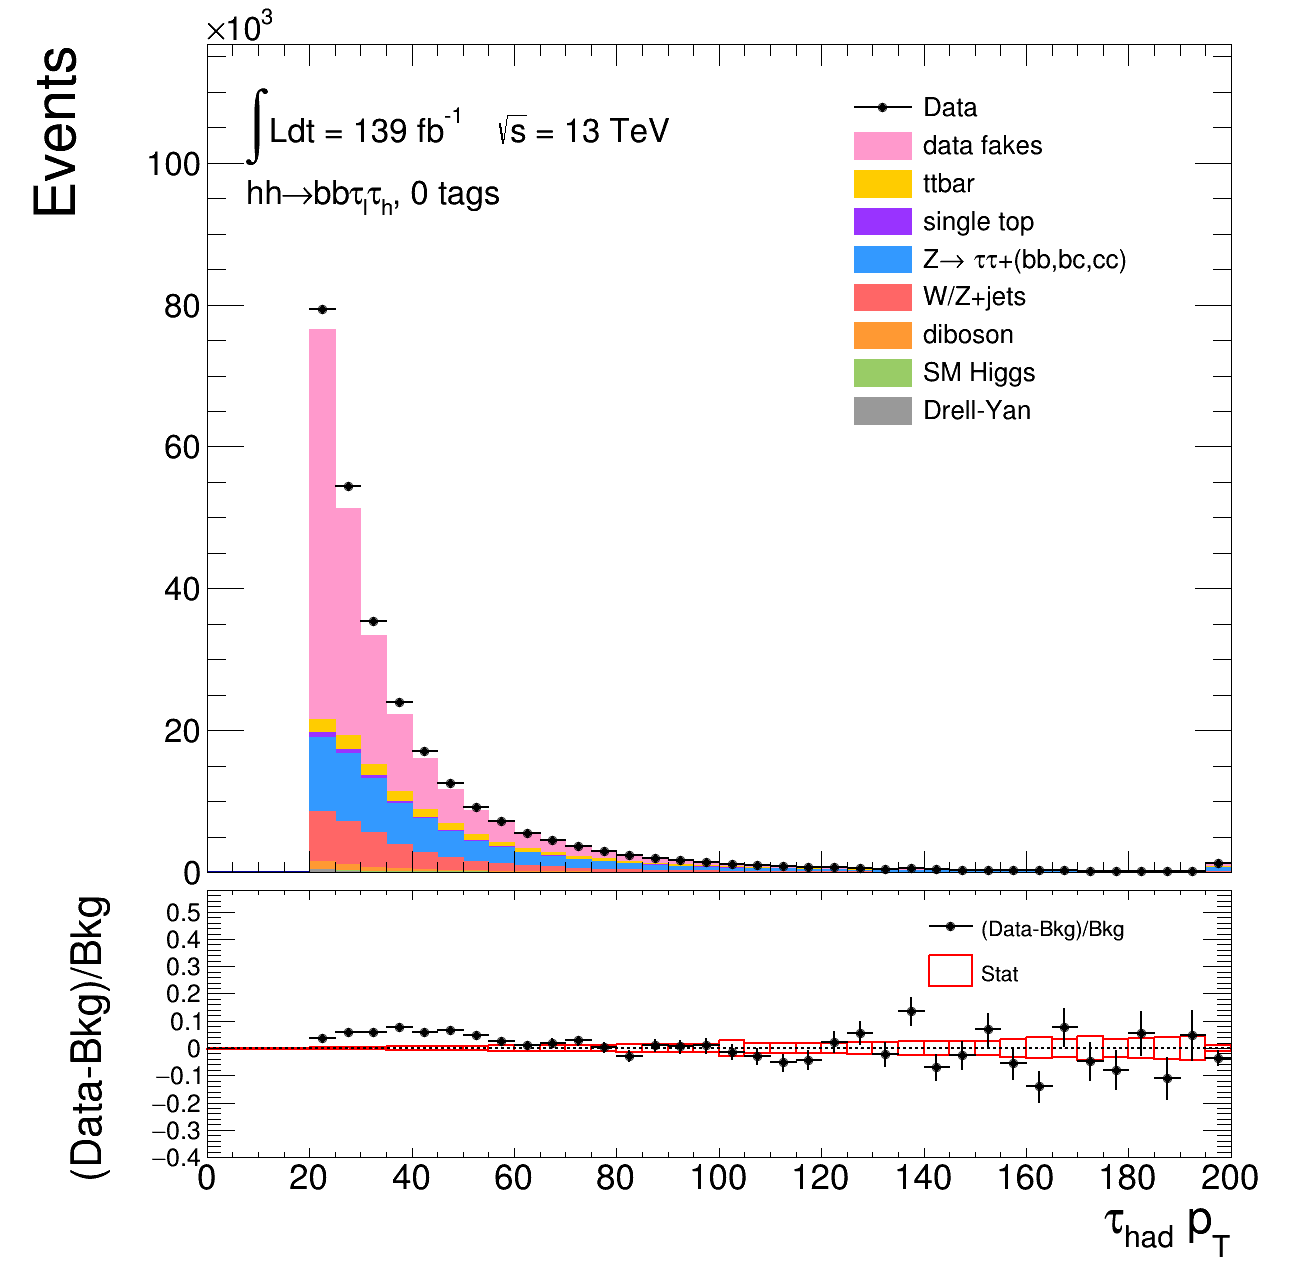
\includegraphics[width=.4\textwidth]{DiHiggs/plots/FF_CRs/SR_SLT_datafakes/HNone/BDTVarsHighMbb/0/C_0tag2pjet_0ptv_TauPt.png}
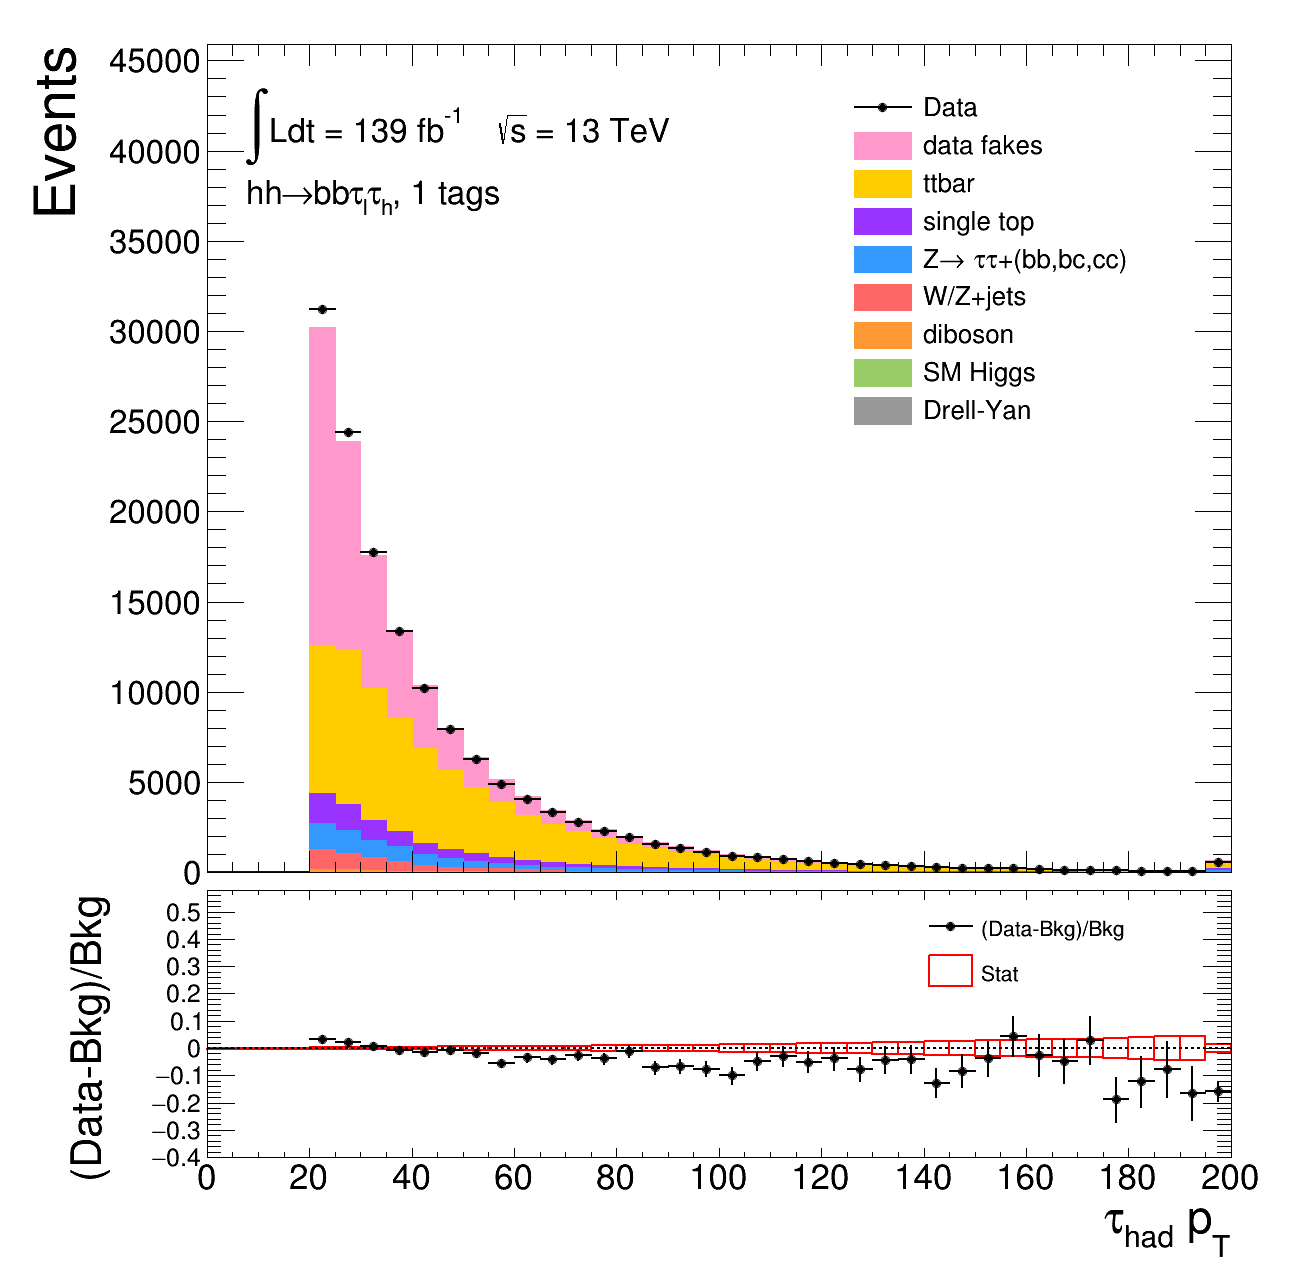
\includegraphics[width=.4\textwidth]{DiHiggs/plots/FF_CRs/SR_SLT_datafakes/HNone/BDTVarsHighMbb/1/C_1tag2pjet_0ptv_TauPt.png} \\
\caption{A comparison of data and background with fakes estimated with combined FF evaluated at the 0-$b$-tagged (left) 
and 1-$b$-tagged region (right) for the SLT channel.
Only statistical uncertainty is considered. }
\label{fig:FFVRSLT}
\end{figure}


\begin{figure}[htbp]
\centering
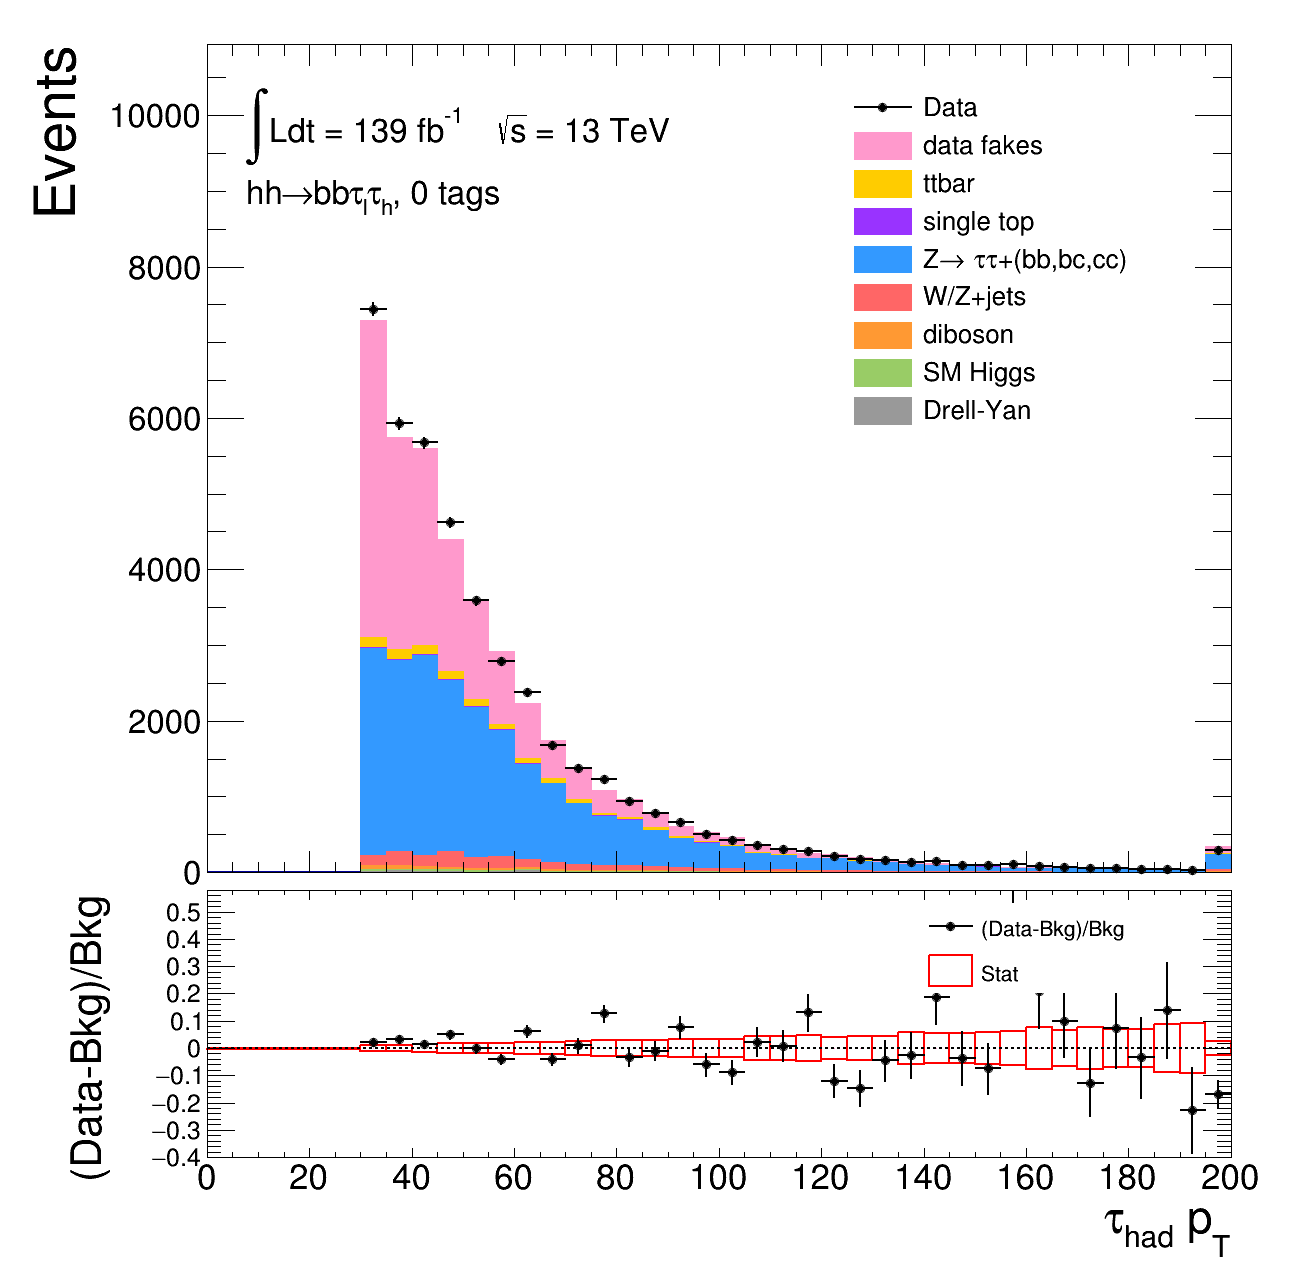
\includegraphics[width=.4\textwidth]{DiHiggs/plots/FF_CRs/SR_LTT_datafakes/HNone/BDTVarsHighMbb/0/C_0tag2pjet_0ptv_TauPt.png}
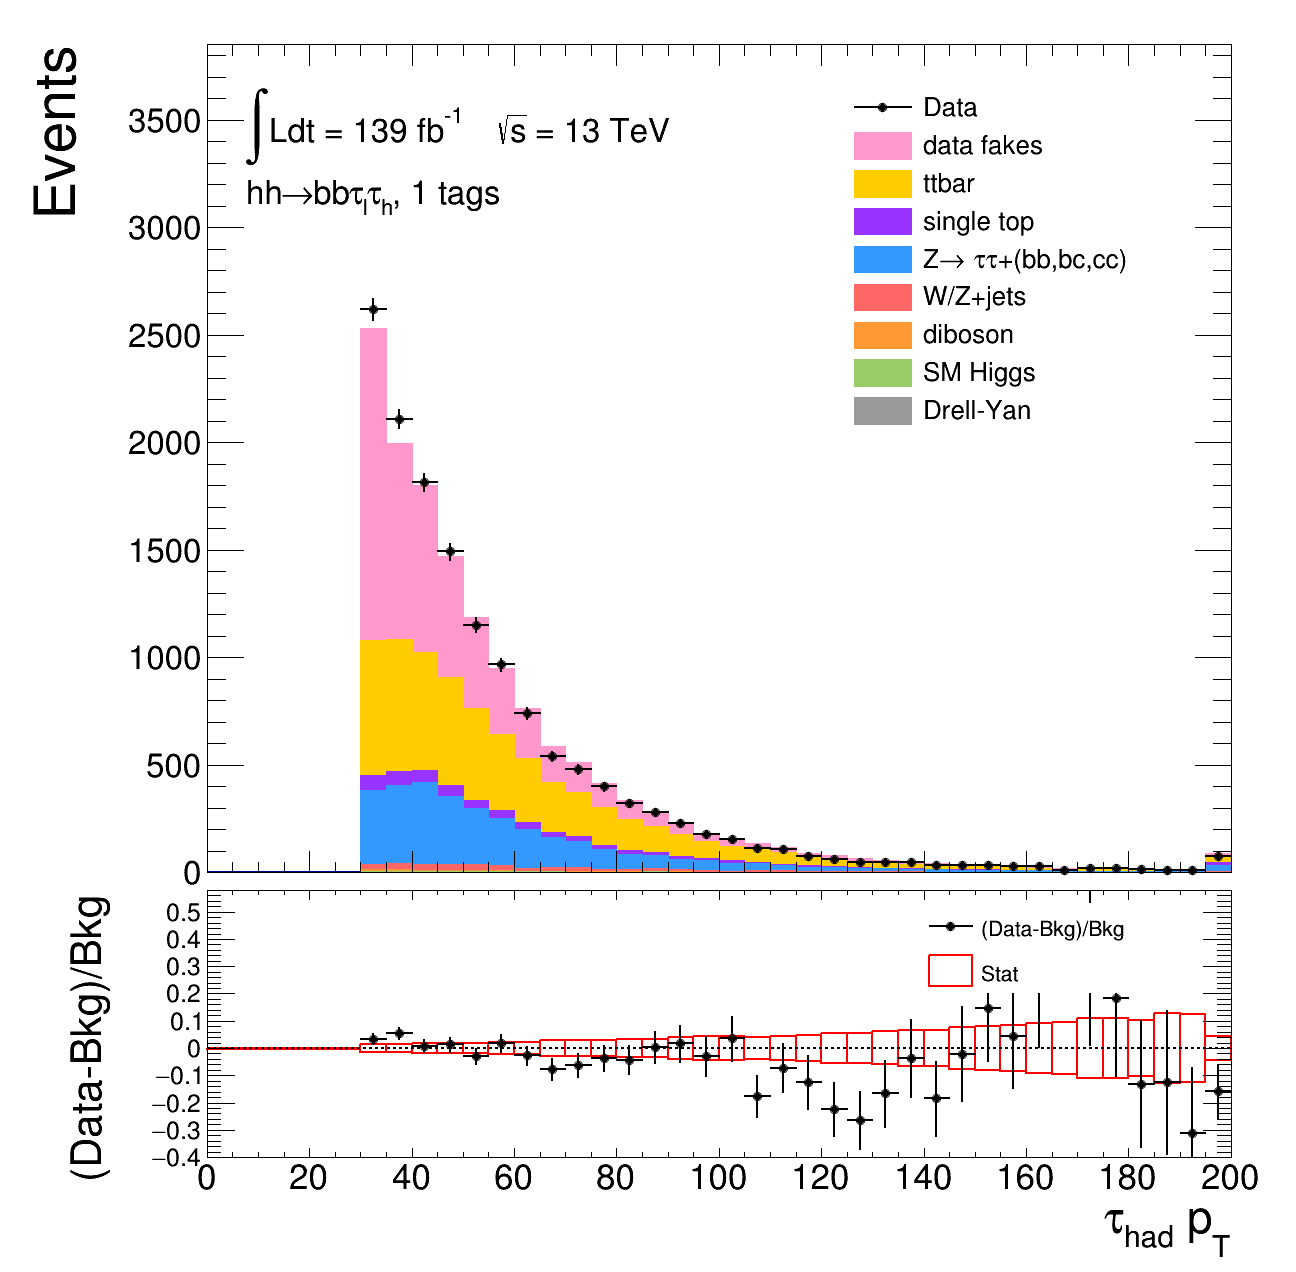
\includegraphics[width=.4\textwidth]{DiHiggs/plots/FF_CRs/SR_LTT_datafakes/HNone/BDTVarsHighMbb/1/C_1tag2pjet_0ptv_TauPt.png} \\
\caption{A comparison of data and background with fakes estimated with combined FF evaluated at the 0-$b$-tagged (left) 
and 1-$b$-tagged region (right) for the LTT channel.
Only statistical uncertainty is considered.  }
\label{fig:FFVRLTT}
\end{figure}









